% Options for packages loaded elsewhere
\PassOptionsToPackage{unicode}{hyperref}
\PassOptionsToPackage{hyphens}{url}
%
\documentclass[
]{book}
\usepackage{amsmath,amssymb}
\usepackage{lmodern}
\usepackage{iftex}
\ifPDFTeX
  \usepackage[T1]{fontenc}
  \usepackage[utf8]{inputenc}
  \usepackage{textcomp} % provide euro and other symbols
\else % if luatex or xetex
  \usepackage{unicode-math}
  \defaultfontfeatures{Scale=MatchLowercase}
  \defaultfontfeatures[\rmfamily]{Ligatures=TeX,Scale=1}
\fi
% Use upquote if available, for straight quotes in verbatim environments
\IfFileExists{upquote.sty}{\usepackage{upquote}}{}
\IfFileExists{microtype.sty}{% use microtype if available
  \usepackage[]{microtype}
  \UseMicrotypeSet[protrusion]{basicmath} % disable protrusion for tt fonts
}{}
\makeatletter
\@ifundefined{KOMAClassName}{% if non-KOMA class
  \IfFileExists{parskip.sty}{%
    \usepackage{parskip}
  }{% else
    \setlength{\parindent}{0pt}
    \setlength{\parskip}{6pt plus 2pt minus 1pt}}
}{% if KOMA class
  \KOMAoptions{parskip=half}}
\makeatother
\usepackage{xcolor}
\usepackage{color}
\usepackage{fancyvrb}
\newcommand{\VerbBar}{|}
\newcommand{\VERB}{\Verb[commandchars=\\\{\}]}
\DefineVerbatimEnvironment{Highlighting}{Verbatim}{commandchars=\\\{\}}
% Add ',fontsize=\small' for more characters per line
\usepackage{framed}
\definecolor{shadecolor}{RGB}{248,248,248}
\newenvironment{Shaded}{\begin{snugshade}}{\end{snugshade}}
\newcommand{\AlertTok}[1]{\textcolor[rgb]{0.94,0.16,0.16}{#1}}
\newcommand{\AnnotationTok}[1]{\textcolor[rgb]{0.56,0.35,0.01}{\textbf{\textit{#1}}}}
\newcommand{\AttributeTok}[1]{\textcolor[rgb]{0.77,0.63,0.00}{#1}}
\newcommand{\BaseNTok}[1]{\textcolor[rgb]{0.00,0.00,0.81}{#1}}
\newcommand{\BuiltInTok}[1]{#1}
\newcommand{\CharTok}[1]{\textcolor[rgb]{0.31,0.60,0.02}{#1}}
\newcommand{\CommentTok}[1]{\textcolor[rgb]{0.56,0.35,0.01}{\textit{#1}}}
\newcommand{\CommentVarTok}[1]{\textcolor[rgb]{0.56,0.35,0.01}{\textbf{\textit{#1}}}}
\newcommand{\ConstantTok}[1]{\textcolor[rgb]{0.00,0.00,0.00}{#1}}
\newcommand{\ControlFlowTok}[1]{\textcolor[rgb]{0.13,0.29,0.53}{\textbf{#1}}}
\newcommand{\DataTypeTok}[1]{\textcolor[rgb]{0.13,0.29,0.53}{#1}}
\newcommand{\DecValTok}[1]{\textcolor[rgb]{0.00,0.00,0.81}{#1}}
\newcommand{\DocumentationTok}[1]{\textcolor[rgb]{0.56,0.35,0.01}{\textbf{\textit{#1}}}}
\newcommand{\ErrorTok}[1]{\textcolor[rgb]{0.64,0.00,0.00}{\textbf{#1}}}
\newcommand{\ExtensionTok}[1]{#1}
\newcommand{\FloatTok}[1]{\textcolor[rgb]{0.00,0.00,0.81}{#1}}
\newcommand{\FunctionTok}[1]{\textcolor[rgb]{0.00,0.00,0.00}{#1}}
\newcommand{\ImportTok}[1]{#1}
\newcommand{\InformationTok}[1]{\textcolor[rgb]{0.56,0.35,0.01}{\textbf{\textit{#1}}}}
\newcommand{\KeywordTok}[1]{\textcolor[rgb]{0.13,0.29,0.53}{\textbf{#1}}}
\newcommand{\NormalTok}[1]{#1}
\newcommand{\OperatorTok}[1]{\textcolor[rgb]{0.81,0.36,0.00}{\textbf{#1}}}
\newcommand{\OtherTok}[1]{\textcolor[rgb]{0.56,0.35,0.01}{#1}}
\newcommand{\PreprocessorTok}[1]{\textcolor[rgb]{0.56,0.35,0.01}{\textit{#1}}}
\newcommand{\RegionMarkerTok}[1]{#1}
\newcommand{\SpecialCharTok}[1]{\textcolor[rgb]{0.00,0.00,0.00}{#1}}
\newcommand{\SpecialStringTok}[1]{\textcolor[rgb]{0.31,0.60,0.02}{#1}}
\newcommand{\StringTok}[1]{\textcolor[rgb]{0.31,0.60,0.02}{#1}}
\newcommand{\VariableTok}[1]{\textcolor[rgb]{0.00,0.00,0.00}{#1}}
\newcommand{\VerbatimStringTok}[1]{\textcolor[rgb]{0.31,0.60,0.02}{#1}}
\newcommand{\WarningTok}[1]{\textcolor[rgb]{0.56,0.35,0.01}{\textbf{\textit{#1}}}}
\usepackage{longtable,booktabs,array}
\usepackage{calc} % for calculating minipage widths
% Correct order of tables after \paragraph or \subparagraph
\usepackage{etoolbox}
\makeatletter
\patchcmd\longtable{\par}{\if@noskipsec\mbox{}\fi\par}{}{}
\makeatother
% Allow footnotes in longtable head/foot
\IfFileExists{footnotehyper.sty}{\usepackage{footnotehyper}}{\usepackage{footnote}}
\makesavenoteenv{longtable}
\usepackage{graphicx}
\makeatletter
\def\maxwidth{\ifdim\Gin@nat@width>\linewidth\linewidth\else\Gin@nat@width\fi}
\def\maxheight{\ifdim\Gin@nat@height>\textheight\textheight\else\Gin@nat@height\fi}
\makeatother
% Scale images if necessary, so that they will not overflow the page
% margins by default, and it is still possible to overwrite the defaults
% using explicit options in \includegraphics[width, height, ...]{}
\setkeys{Gin}{width=\maxwidth,height=\maxheight,keepaspectratio}
% Set default figure placement to htbp
\makeatletter
\def\fps@figure{htbp}
\makeatother
\setlength{\emergencystretch}{3em} % prevent overfull lines
\providecommand{\tightlist}{%
  \setlength{\itemsep}{0pt}\setlength{\parskip}{0pt}}
\setcounter{secnumdepth}{5}
\usepackage{booktabs}
\ifLuaTeX
  \usepackage{selnolig}  % disable illegal ligatures
\fi
\usepackage[]{natbib}
\bibliographystyle{plainnat}
\IfFileExists{bookmark.sty}{\usepackage{bookmark}}{\usepackage{hyperref}}
\IfFileExists{xurl.sty}{\usepackage{xurl}}{} % add URL line breaks if available
\urlstyle{same} % disable monospaced font for URLs
\hypersetup{
  pdftitle={Visualisation for bioacoustics and ecoacoustics in R},
  pdfauthor={Ed Baker},
  hidelinks,
  pdfcreator={LaTeX via pandoc}}

\title{Visualisation for bioacoustics and ecoacoustics in R}
\author{Ed Baker}
\date{2022-10-29}

\begin{document}
\maketitle

{
\setcounter{tocdepth}{1}
\tableofcontents
}
\hypertarget{about}{%
\chapter*{About}\label{about}}
\addcontentsline{toc}{chapter}{About}

Bioacoustics and ecoacoustics are rapidly advancing multi-disciplinary fields of study that focus on how organisms communicate using sound, and the overall sound of a landscape (the soundscape). Despite the focus on sound, much of the communication of ideas, and even sounds, between researchers is done using graphical representations.

This should not come as a surprise, the printing press came centuries before the radio as a means for long distance communication, and ink on paper has a permanence that sounds would not achieve for a long time after the invention of writing. The current flourishing of these disciplines is driven as much by the low cost and ease of use of products such as AudioMoth and the decreasing cost of digitial storage and processing as by novel ideas.

Visualizations of acoustic data however are not going away - we are a predominantly visual species, and as ways of summarising acoustic data - or making the ultrasound tangible, they are powerful tools in the hands of the acoustician.

\hypertarget{intro}{%
\chapter{Introduction}\label{intro}}

\begin{quote}
``\ldots while we take it for granted that sounds may be described visually, the convention is recent, is by no means universal and, as I will show, is in many ways dangerous and inappropriate.''

\hfill --- \citet{schafer1977}
\end{quote}

While Murray Schafer's \emph{Tuning of the World} \citep{schafer1977} inspired many soundscape scientists, this view is of an earlier time, where the concept of multiple simultaneous streams of acoustic data being processed by a single individual was still an idea beyond the horizon. Individual sounds could be isolated and studied (as today they still are by bioacousticians interested in the behaviour of individual species). The scale of many contemporary ecoacoustics projects precludes an individual from listening to every minute that is recorded, the task no longer delegated to students but networks of machines.

Additionally, it is now useful to distinguish between two concepts that Schafer bought together under the concept of \emph{notation}. Schafer used this term to bring together what is more typically known as notation -- phonetics and musical notation -- alongside visual representations of the physical properties of acoustic waves (amplitude, frequency, etc).

Historically both musical notation and phonemes have been used to describe the songs of various animals, however these methods do not scale to the entirety of the biological soundscape. There is after all, a great deal of the soundscape that is beyond the limits of human hearing, the infrasound, the ultrasound, and the quiet. All manner of information is gathered and shared by other species beyond the limits of our perception, and visualisation is the main tool by which we are able to interpret the entire soundscape. For all species that share it.

\hypertarget{predominance-of-the-visual}{%
\section{Predominance of the visual}\label{predominance-of-the-visual}}

\hypertarget{basic-acoustic-terminology}{%
\section{Basic acoustic terminology}\label{basic-acoustic-terminology}}

\hypertarget{types-of-files}{%
\section{Types of files}\label{types-of-files}}

Even though the costs of digital storage have fallen significantly (Figure \ref{fig:storage-costs}) the cost of file transfer and storage are still significant factors in many acoustics projects. For this reason it is sometimes necessary to compress the audio file in some way: discarding some data in exchange for cost reductions.

\begin{figure}

{\centering 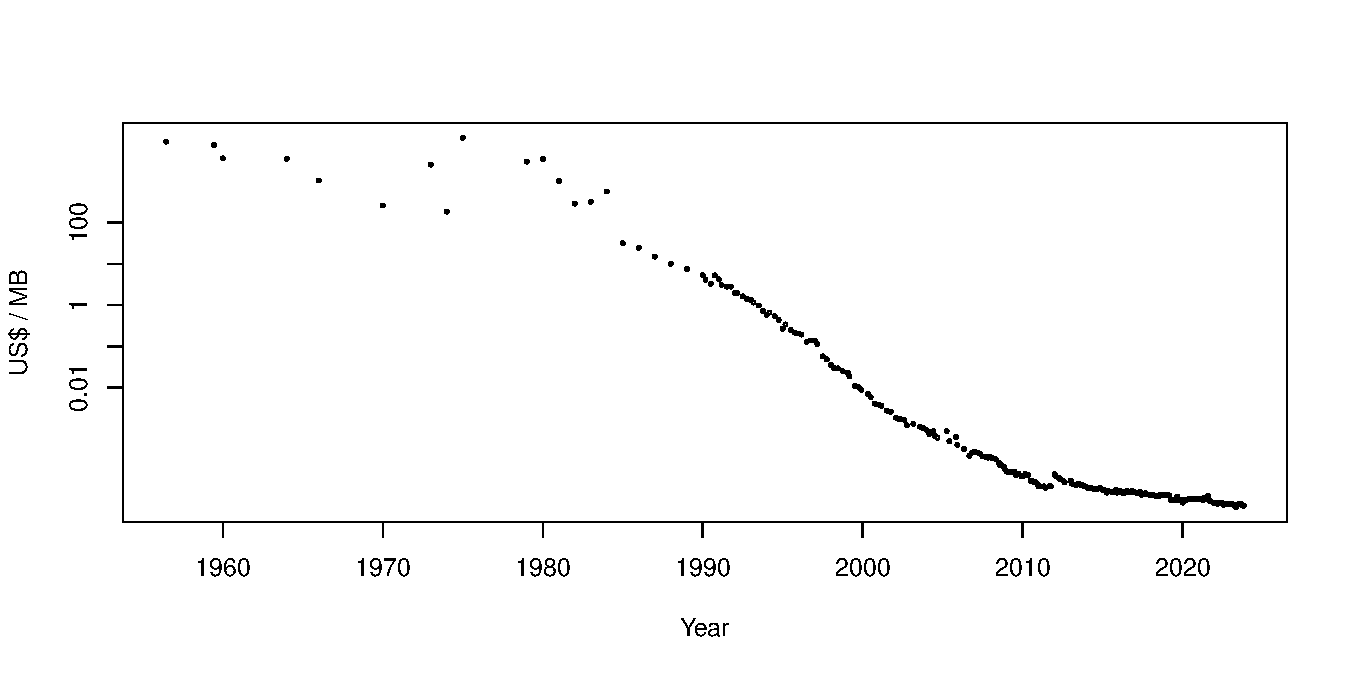
\includegraphics[width=0.9\linewidth]{_main_files/figure-latex/storage-costs-1} 

}

\caption{Storage costs per megabyte over time. Data from https://jcmit.net/diskprice.htm.}\label{fig:storage-costs}
\end{figure}

This process of compression may affect visualisation of the audio files, or even the types of visualisation that are possible for a given file.

\hypertarget{uncompressed-waveform-files}{%
\subsection{Uncompressed waveform files}\label{uncompressed-waveform-files}}

Waveform files are created by sampling the amplitude at a sensor at a constant rate, typically tens of thousands of times per second (Figure \ref{fig:wave-sampling}).

\begin{figure}

{\centering 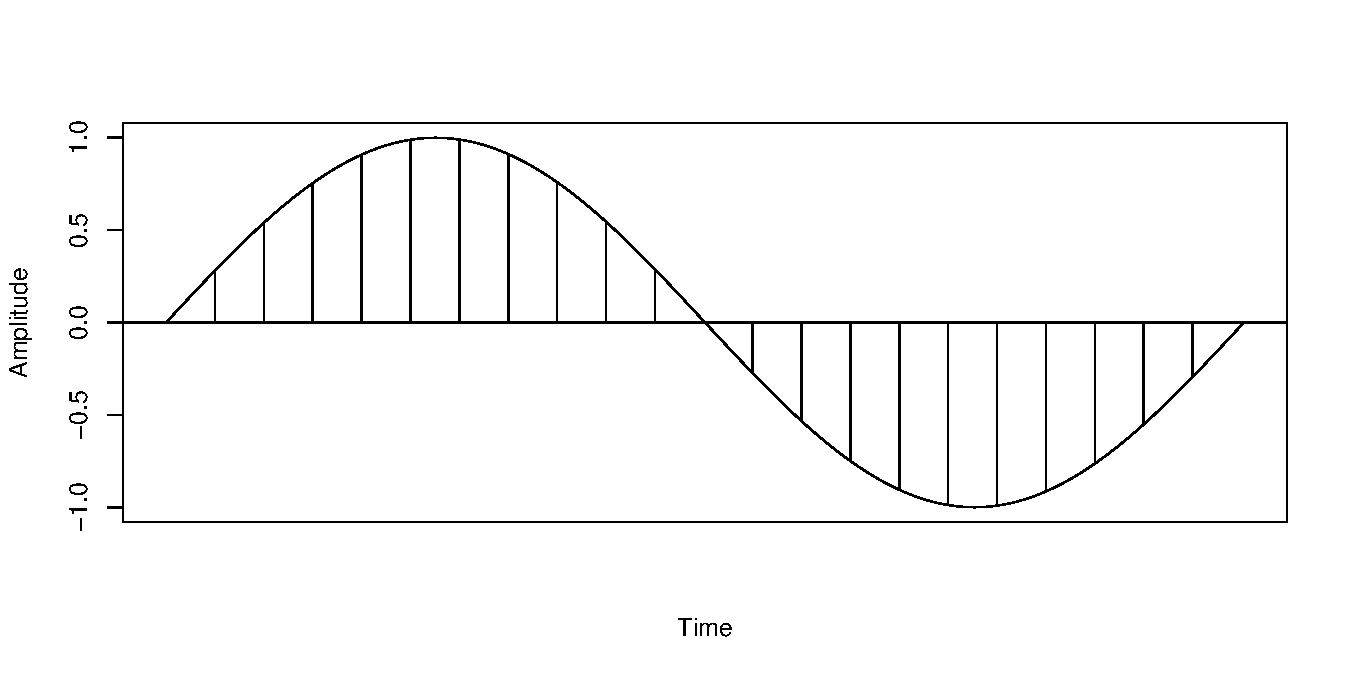
\includegraphics[width=0.9\linewidth]{_main_files/figure-latex/wave-sampling-1} 

}

\caption{Sampling a waveform.}\label{fig:wave-sampling}
\end{figure}

This is achieved using an analogue-to-digital converter (DAC) that converts the continuous variations in amplitude into a number of discrete levels that can be represented numerically (Figure \ref{fig:sampled-wave}. The number of discrete levels is dependant on the analogue-to-digitial converter (ADC), a typical 16-bit depth has \(2^{16}=65536\) possible values.

The

\begin{figure}

{\centering 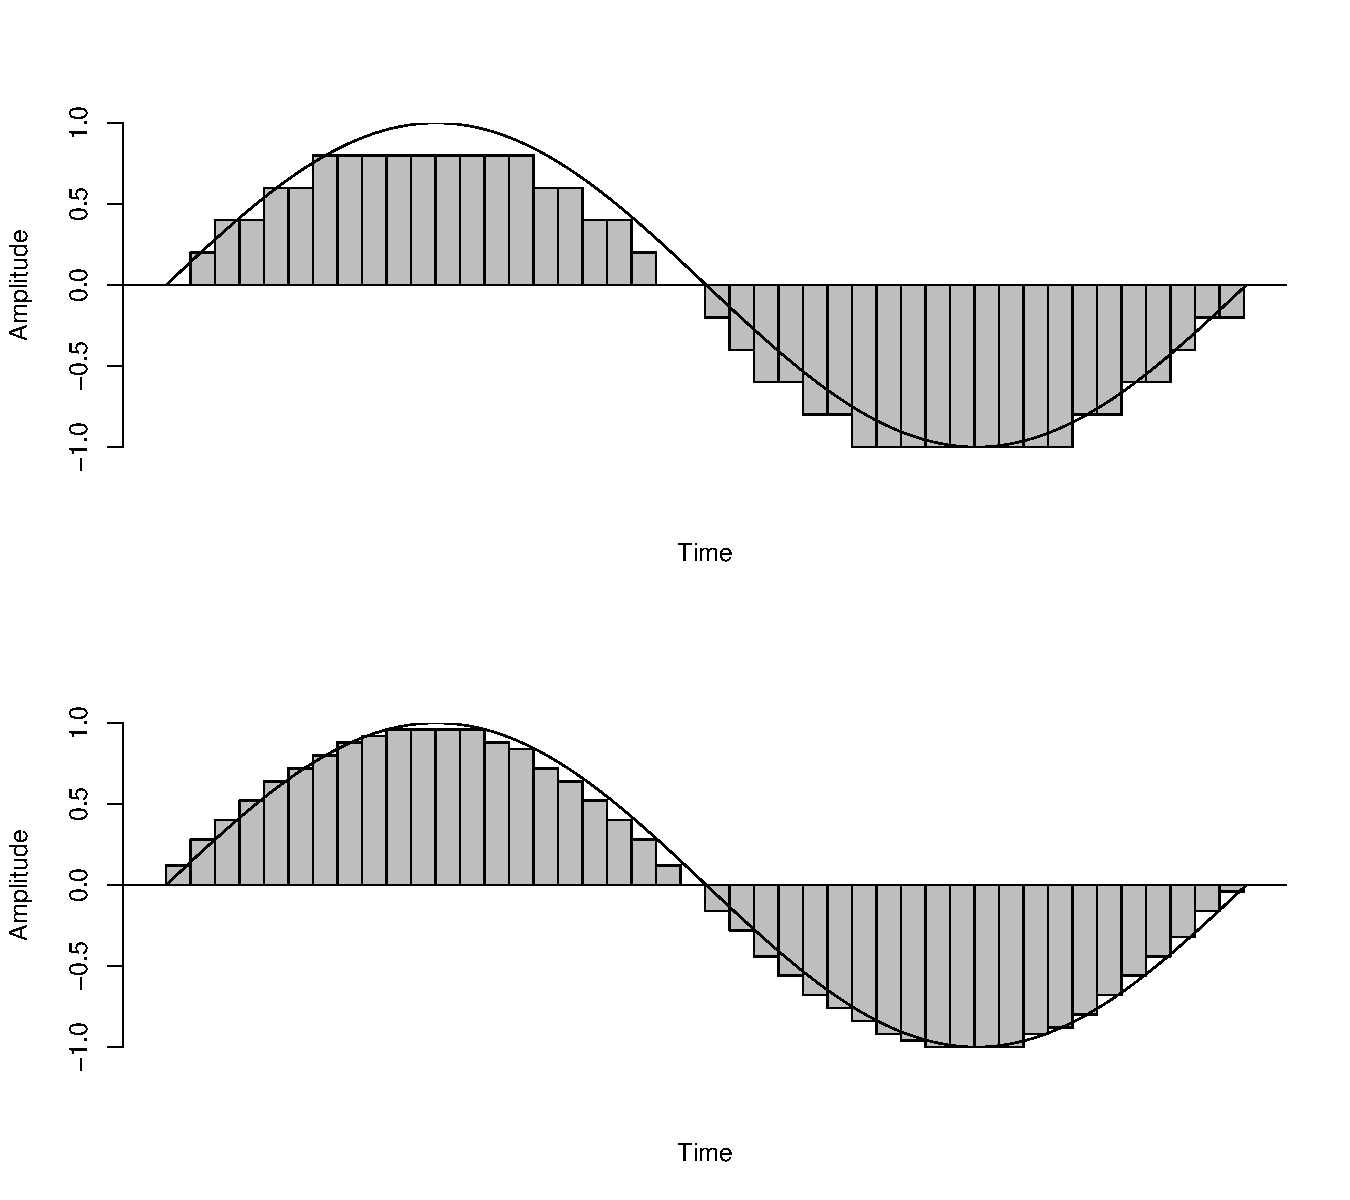
\includegraphics[width=0.9\linewidth]{_main_files/figure-latex/sampled-wave-1} 

}

\caption{A sampled waveform with low bit depth (top) and higher bit depth(bottom).}\label{fig:sampled-wave}
\end{figure}

\hypertarget{lossy-compression}{%
\subsection{Lossy compression}\label{lossy-compression}}

\hypertarget{zero-crossing-files}{%
\subsection{zero-crossing}\label{zero-crossing-files}}

\hypertarget{history}{%
\chapter{History}\label{history}}

\hypertarget{goals-of-visualisation}{%
\section{Goals of visualisation}\label{goals-of-visualisation}}

Visualisation of acoustic information may be performed for a number of reasons. Purely descriptive graphical representations may have the goal of invoking in the mind the sound that is being represented, allowing knowledge of how somethng sounds to be passed from one mind to another via visual media.

\begin{quote}
``I have frequently experimented with graphic notations, and in the course of these experiments it has occurred to me that a new type of artistic experience may be opening up to us, in which musical clements could have revitalized graphic correspondences in such a way that one sensation could be triggered by another to produce synaesthesia - that is, a fusion of two art forms into a unitary experience.''

\hfill --- \citep{schafer1975}
\end{quote}

While it may be argued that the decreasing costs of electronic data storage and transmission remove the need for converting audio into graphical form, these trends contribute to an increased abundance and availability of acoustic data. It is normally the case that it is quicker and easier to scan this large quantity of acoustic information when it is represented visually than by listening to it (Figure \ref{fig:quicker-visually}).

\begin{figure}

{\centering 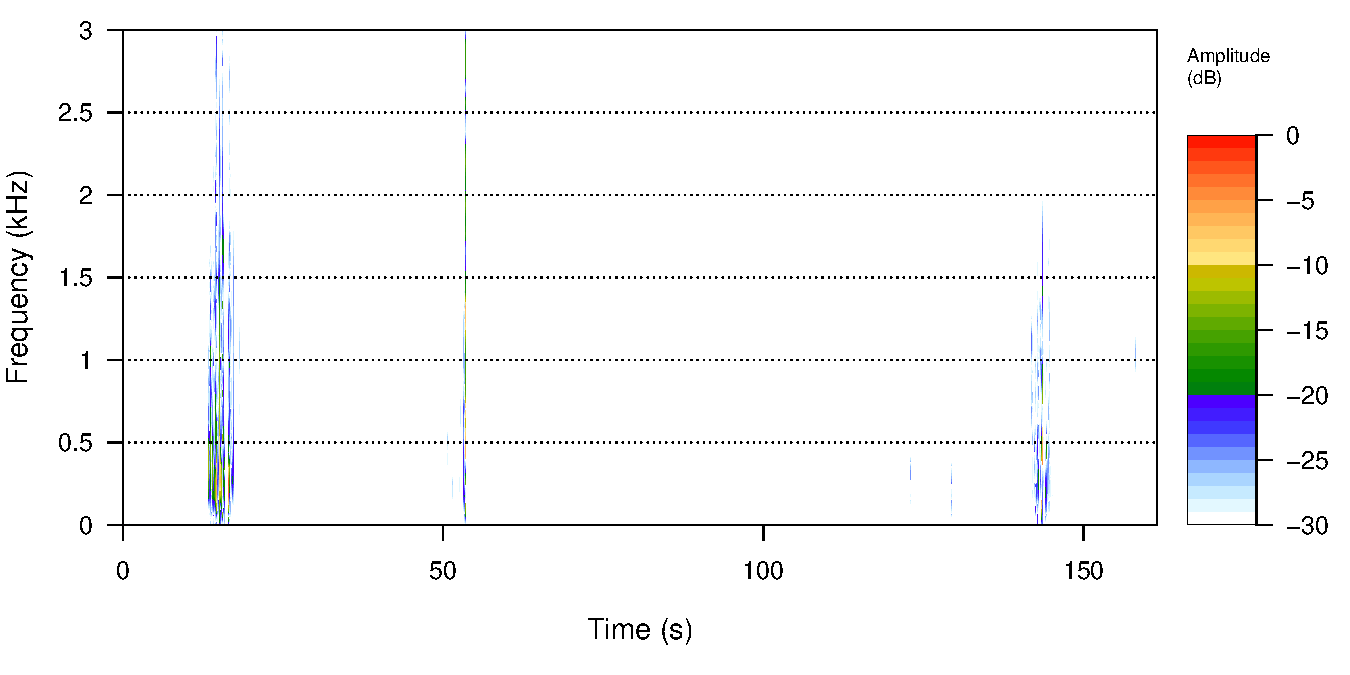
\includegraphics[width=0.9\linewidth]{_main_files/figure-latex/quicker-visually-1} 

}

\caption{Even for a short file of three minutes duration it is quicker to identify regions of interest visually than by listening.}\label{fig:quicker-visually}
\end{figure}

It should also be said that many current machine learning techniques used in acoustics work upon data that has initially been converted into graphical form. Is this an optimum method, or just a consequence of the Predominance of the Visual?

\hypertarget{descriptive-acoustics}{%
\section{Descriptive acoustics}\label{descriptive-acoustics}}

\hypertarget{phonemes-and-onomatopoeia}{%
\subsection{Phonemes and onomatopoeia}\label{phonemes-and-onomatopoeia}}

\hypertarget{musical-notation}{%
\subsection{Musical notation}\label{musical-notation}}

Typical musical notation shows broad similarities with a typical audio visualisation familiar to all bioacousticians and ecoacousticians - the frequency against time plot. Time proceeds in a strictly linear fashion from left to right, and frequency is represented rising from bottom to top.

\hypertarget{analytic-acoustics}{%
\section{Analytic acoustics}\label{analytic-acoustics}}

\hypertarget{the-big-three}{%
\subsection{The `big-three'}\label{the-big-three}}

\hypertarget{amplitude-vs-time}{%
\subsubsection{Amplitude vs Time}\label{amplitude-vs-time}}

\hypertarget{ampltiude-vs-frequency}{%
\subsubsection{Ampltiude vs Frequency}\label{ampltiude-vs-frequency}}

\hypertarget{frequency-vs-time}{%
\subsubsection{Frequency vs Time}\label{frequency-vs-time}}

\hypertarget{early-viz}{%
\chapter{Early visualisations - the analog years}\label{early-viz}}

\hypertarget{crts}{%
\section{CRTs}\label{crts}}

\hypertarget{print-outs}{%
\section{Print outs}\label{print-outs}}

\hypertarget{static-digital-images}{%
\chapter{Static digital images}\label{static-digital-images}}

The three basic quantities of sound waves are time, frequency, and amplitude. The most commonly used visualisations of sounds are consequently combinations of these properties.

The \texttt{seewave} package \citep{seewave} is the easiest way to produce these plots, and we will use the \texttt{sheep} audio sample provided by \texttt{seewave} for the first plots.

\begin{Shaded}
\begin{Highlighting}[]
\FunctionTok{library}\NormalTok{(seewave)}
\FunctionTok{data}\NormalTok{(sheep, }\AttributeTok{package=}\StringTok{"seewave"}\NormalTok{)}
\end{Highlighting}
\end{Shaded}

\hypertarget{the-time-domain}{%
\section{The time domain}\label{the-time-domain}}

The \emph{time domain} is used to describe acoustic analyses where the recorded waveform is not analysed for frequency. Conversion of a waveform to a spectrum of frequencies is a relatively costly computation and, before digital computers, hard to achieve with the precision and resolution we are accustomed to today.

\hypertarget{oscillograms}{%
\subsection{Oscillograms}\label{oscillograms}}

Digitally sampled audio is a series of amplitude measurements, sampled at a regular time time interval. Given that it now seems natural for time to be expressed on the x axis, increasing towards the right, the most basic plot we could recreate from a sampled file would be plotting amplitude values against time.

\begin{figure}

{\centering 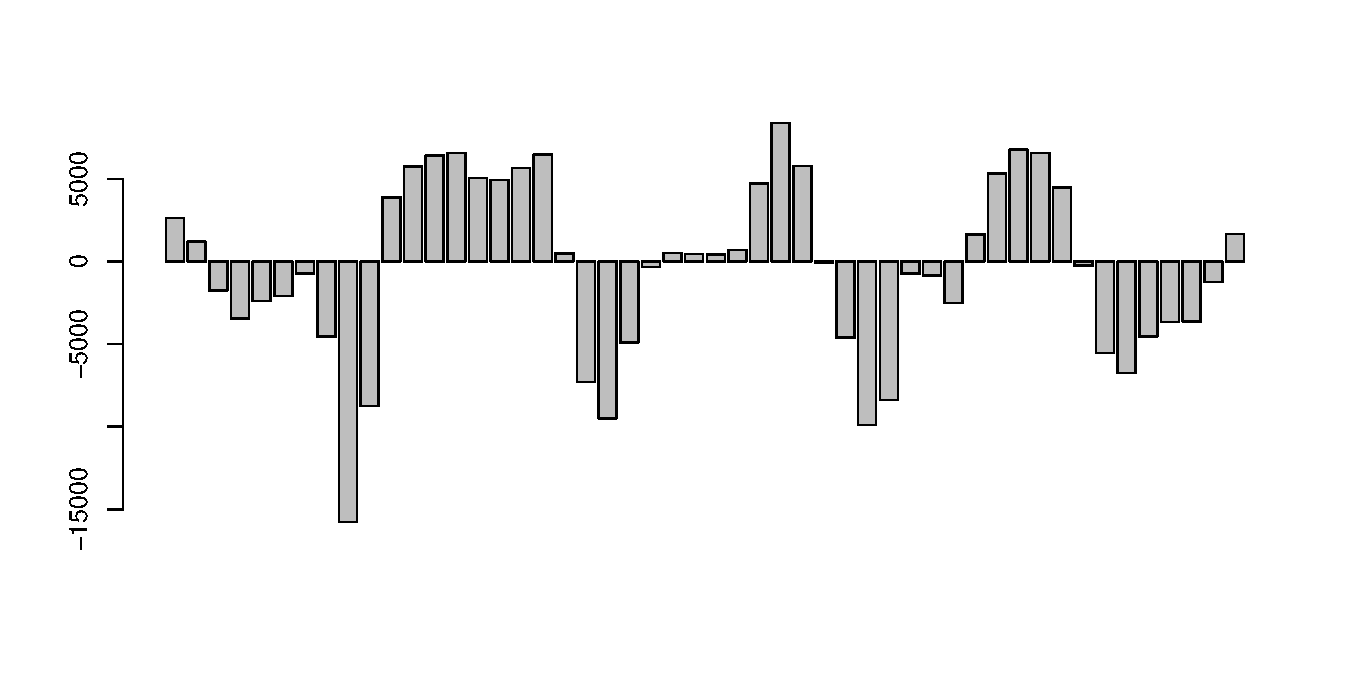
\includegraphics[width=0.9\linewidth]{_main_files/figure-latex/amplitude-bars-1} 

}

\caption{Plotting a waveform}\label{fig:amplitude-bars}
\end{figure}

Figure \ref{fig:amplitude-bars} shows 50 samples from the \texttt{sheep} audio file plotted using the standard R \texttt{barplot()} function. This representation has the advantage that the individual bars ar a visual reminder that we are handling a sampled representation, as opposed to a continuously varying waveform. It is common however to create a visual representation closer to that of an actual wave (Figure @ref(fig:amplitude-lines shows how this is achieved using base R functions).

\begin{figure}

{\centering 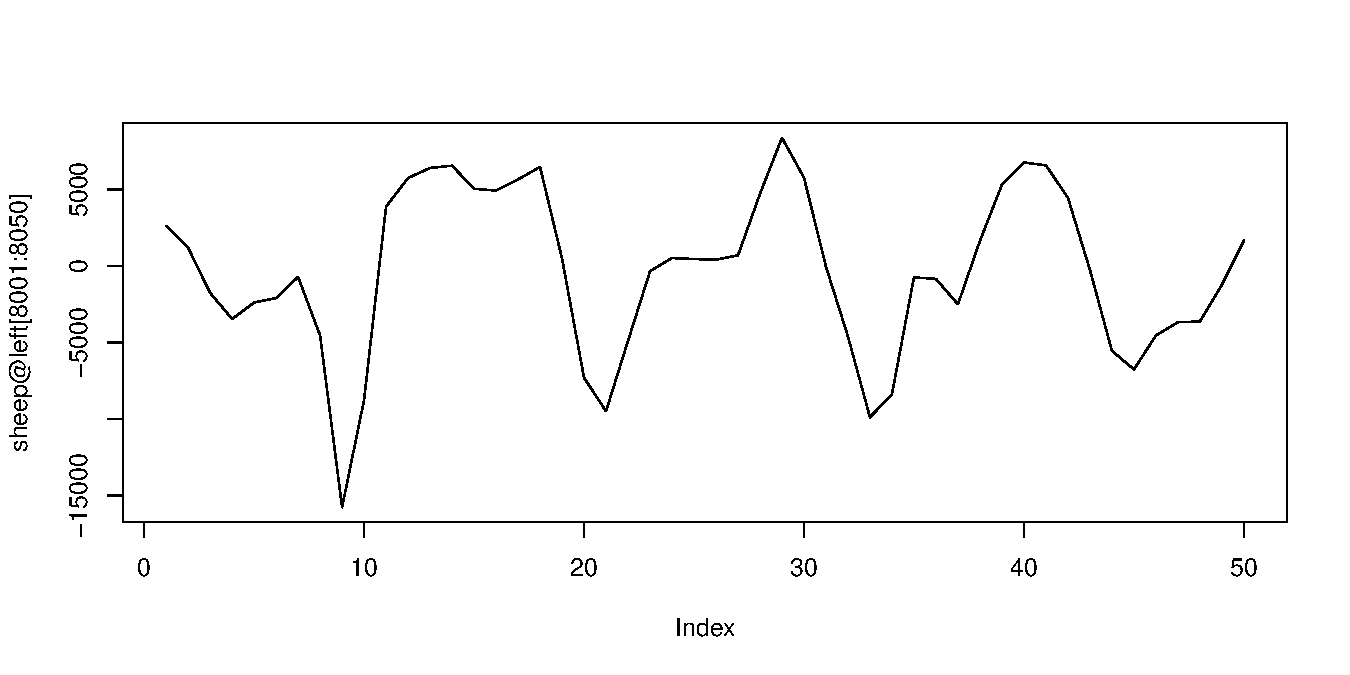
\includegraphics[width=0.9\linewidth]{_main_files/figure-latex/amplitude-lines-1} 

}

\caption{Plotting a waveform}\label{fig:amplitude-lines}
\end{figure}

The \texttt{oscillo()} function from \texttt{seewave} handles the labelling of axes for us, and is a very convenient solution. Figure \ref{fig:amplitude-oscillo} shows the resulting plot, an oscillogram, for the entire \texttt{sheep} file.

\begin{figure}

{\centering 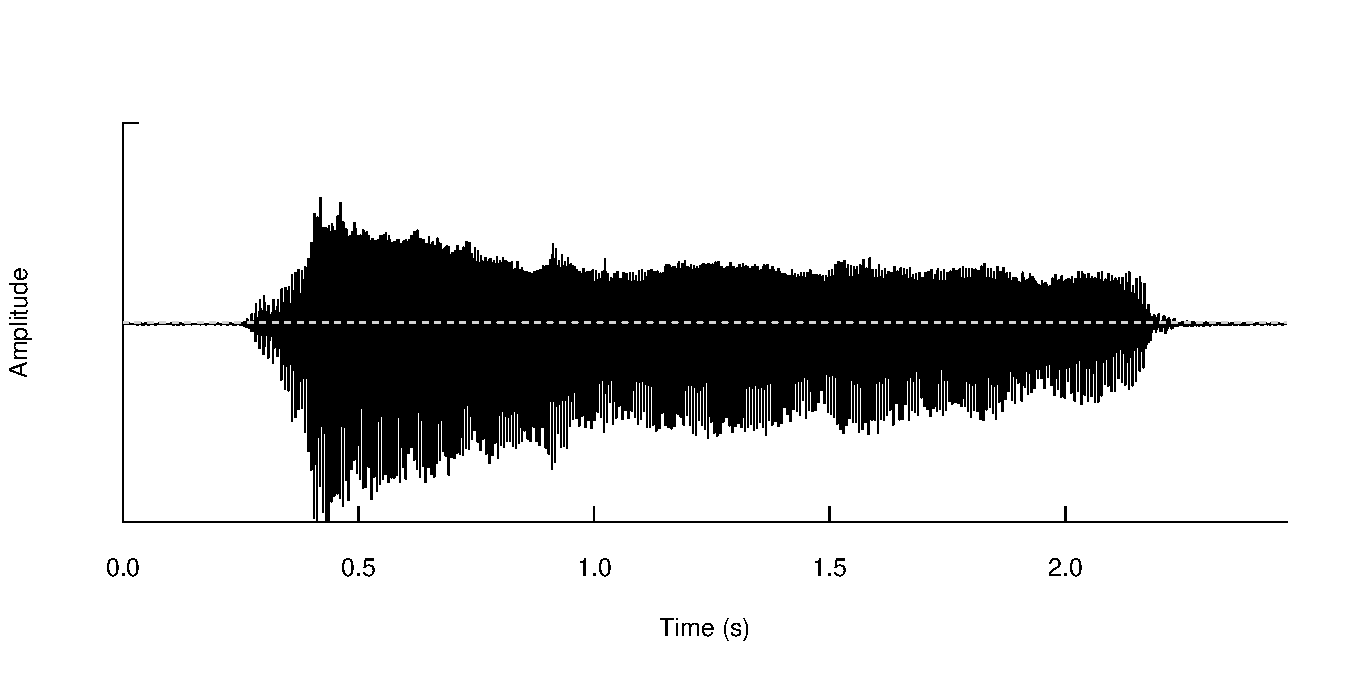
\includegraphics[width=0.9\linewidth]{_main_files/figure-latex/amplitude-oscillo-1} 

}

\caption{Oscillogram}\label{fig:amplitude-oscillo}
\end{figure}

\hypertarget{the-frequency-domain}{%
\section{The frequency domain}\label{the-frequency-domain}}

The \emph{frequency domain} covers analyses in which frequency data is extracted from the sampled waveform. This information is generally extracted using the \emph{Fast Fourier Transform} algorithm.

\hypertarget{plotting-a-spectrum}{%
\subsection{Plotting a spectrum}\label{plotting-a-spectrum}}

A spectrum is a plot of amplitude against frequency.

\begin{figure}

{\centering 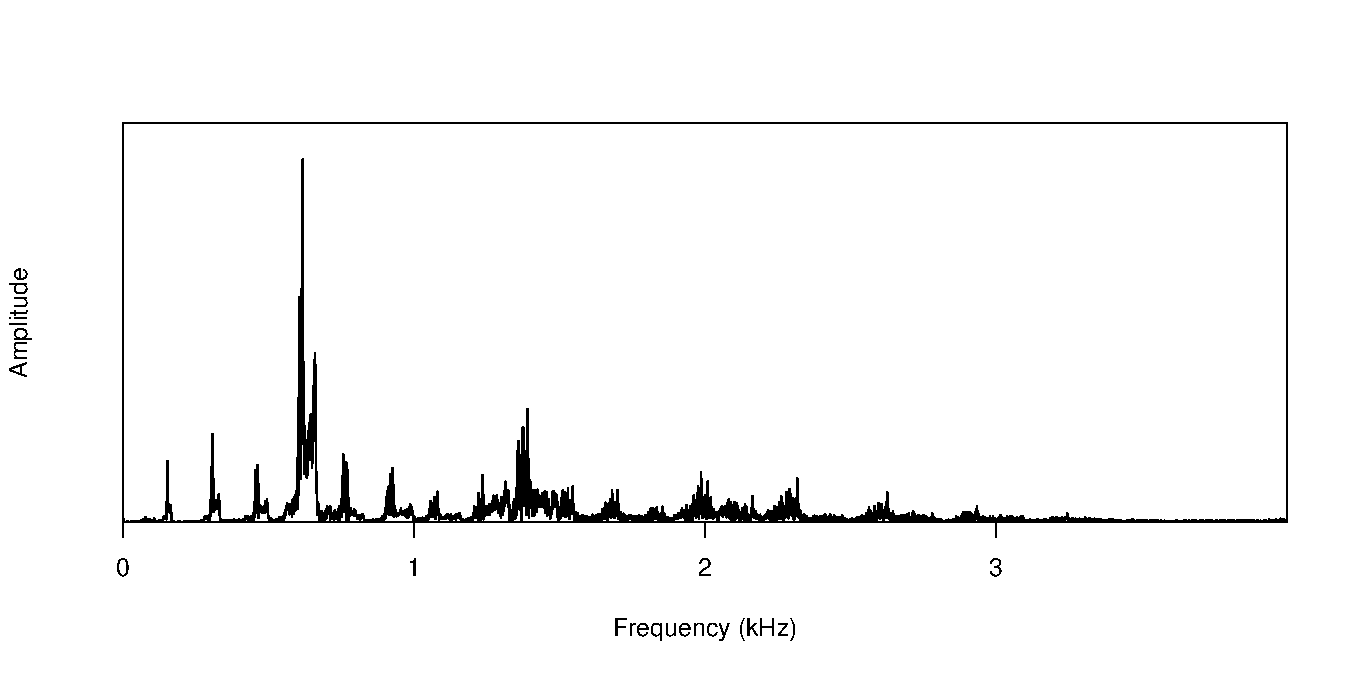
\includegraphics[width=0.9\linewidth]{_main_files/figure-latex/spectrum-1} 

}

\caption{Spectrum}\label{fig:spectrum}
\end{figure}

\hypertarget{plotting-a-spectrogram}{%
\subsection{Plotting a spectrogram}\label{plotting-a-spectrogram}}

\begin{figure}

{\centering 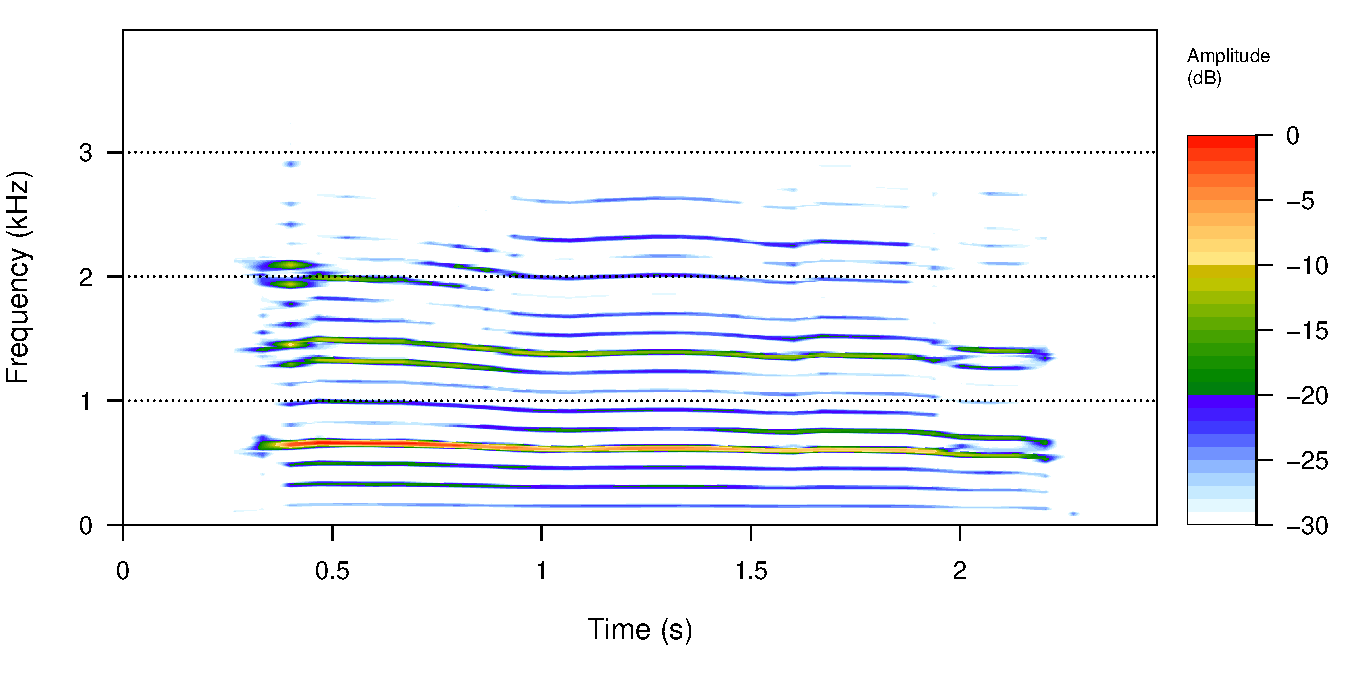
\includegraphics[width=0.9\linewidth]{_main_files/figure-latex/spectrogram-1} 

}

\caption{Spectrogram}\label{fig:spectrogram}
\end{figure}

\hypertarget{settings-for-a-fft}{%
\subsubsection{Settings for a FFT}\label{settings-for-a-fft}}

\hypertarget{dynamic-digital-visualisations}{%
\chapter{Dynamic digital visualisations}\label{dynamic-digital-visualisations}}

\hypertarget{video-spectrograms}{%
\section{Video spectrograms}\label{video-spectrograms}}

\hypertarget{zcjs-zero-crossing-file-visualisation}{%
\section{zcjs: Zero-crossing File Visualisation}\label{zcjs-zero-crossing-file-visualisation}}

The zcjs JavaScript library was originally developed for displaying zero-crossing audio files (\ref{zero-crossing-files}) on the web as part of the BioAcoustica project (\url{https://bio.acousti.ca}; \citet{baker2015bioacoustica}). The \texttt{zcjs} package \citep{zcjsr} imports this visualisation functionality into R.

The following code installs the \texttt{zcjs} package.

\begin{Shaded}
\begin{Highlighting}[]
\FunctionTok{install.packages}\NormalTok{(}\StringTok{"devtools"}\NormalTok{)}
\NormalTok{devtools}\SpecialCharTok{::}\FunctionTok{install\_github}\NormalTok{(}\StringTok{"bioacoustica/zcjs{-}r"}\NormalTok{)}
\end{Highlighting}
\end{Shaded}

To load the package:

\begin{Shaded}
\begin{Highlighting}[]
\FunctionTok{library}\NormalTok{(zcjs)}
\end{Highlighting}
\end{Shaded}

The package comes with a demonstration file for testing the package's functionality.

\hypertarget{customising-a-zcjs-plot}{%
\subsection{Customising a zcjs plot}\label{customising-a-zcjs-plot}}

\textbf{x-compress}

\hypertarget{representing-soundscapes}{%
\chapter{Representing Soundscapes}\label{representing-soundscapes}}

\hypertarget{false-colour-index-spectrograms}{%
\section{False Colour Index Spectrograms}\label{false-colour-index-spectrograms}}

\hypertarget{patterns-of-activity}{%
\chapter{Patterns of activity}\label{patterns-of-activity}}

Lots of organismal activities are tied to the cycles of the day, and particularly in temperate zones, cycles of the year. These cycles bring regular fluctuations in light levels, day lengths, temperatures, and a host of other influences. Often these cycles interact, with the dawn chorus peaking in the early daylight hours, and it's timing and intensity fluctuating on a yearly cycle. This chapter looks at visualising these cycles, and additionally the effects of lunar cycles.

These plots are created using the SonicScrewdriver package \citep{sonicscrewdriver} which in turn uses the suncalc package \citep{suncalc} to perform the required sun and moon position calculations. The Plotrix package \citep{plotrix} is used for creating the visualisation. These packages can be installed as shown below.

\begin{Shaded}
\begin{Highlighting}[]
\FunctionTok{install.packages}\NormalTok{(}\FunctionTok{c}\NormalTok{(}\StringTok{"plotrix"}\NormalTok{, }\StringTok{"sonicscrewdriver"}\NormalTok{))}
\end{Highlighting}
\end{Shaded}

The SonicScrewdriver package must be loaded before constructing a visual.

\begin{Shaded}
\begin{Highlighting}[]
\FunctionTok{library}\NormalTok{(sonicscrewdriver)}
\end{Highlighting}
\end{Shaded}

\hypertarget{daily-cycles}{%
\section{Daily Cycles}\label{daily-cycles}}

The use of the term \emph{diel} for daily cycles has been contested by \citet{broughton1963} as being an incorrectly formed unnecessary neologism, it sees greater use (according to the online Oxford English Dictionary) than his suggested \emph{nycthemeral}.

The design for these plots came from a desire to compare the dawn chorus at various locations around the UK, although they also offer great potential for comparing locations with greater longitudinal and/or latitudinal separation. The plots show the times of day, night, twilight (\ref{twilight-types}), sunrise, sunset, nadir and solar noon. The day part of the plot shows the altitude (angle of the sun above the horizon) throughout the day, with the maximum value representing the sun being directly overhead.

\hypertarget{twilight-types}{%
\subsection{The Types of Twilight}\label{twilight-types}}

\begin{figure}

{\centering 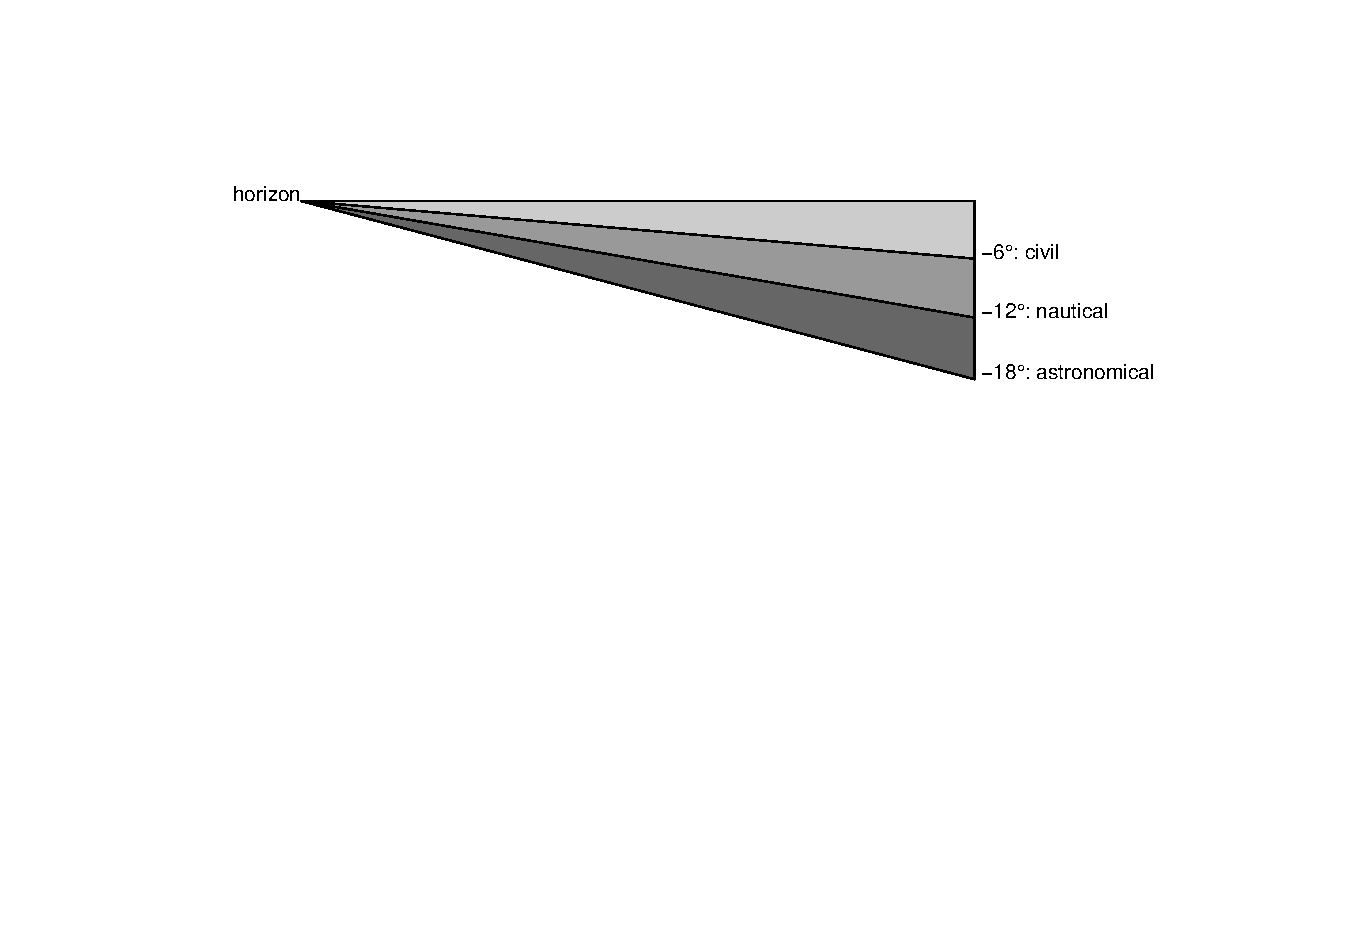
\includegraphics[width=0.9\linewidth]{_main_files/figure-latex/twilights-1} 

}

\caption{Different types of twilight as the sun sets below the horizon}\label{fig:twilights}
\end{figure}

\hypertarget{civil-twilight}{%
\subsubsection{Civil Twilight}\label{civil-twilight}}

Civil twilight occurs when the geometric centre of the sun (as seen from Earth) passes between 0° and 6° below the horizon. During this time it is normal for humans not to need the assistance of artifical light for everyday tasks.

\hypertarget{nautical-twilight}{%
\subsubsection{Nautical Twilight}\label{nautical-twilight}}

Nautical twilight occurs when the sun is between 6° and 12° below the horizon. During this time there is sufficient light to distinguish the horizon even without illumination from the moon (allowing determination of position at sea through star sightings).

\hypertarget{astronomical-twilight}{%
\subsubsection{Astronomical Twilight}\label{astronomical-twilight}}

When the sun is between 12° and 18° below the horizon many astronomical observations are possible even though some light from the sun is visible through the atmosphere. In urban areas with light pollution this is often considered to be a dark sky.

\hypertarget{diel-plots}{%
\subsection{Diel Plots}\label{diel-plots}}

As the times of the solar day are dependent both on the date and location these must be passed to the \texttt{dielPlot()} function.

\begin{Shaded}
\begin{Highlighting}[]
\FunctionTok{dielPlot}\NormalTok{(}\StringTok{"2022{-}08{-}08"}\NormalTok{, }\AttributeTok{lat=}\DecValTok{53}\NormalTok{, }\AttributeTok{lon=}\FloatTok{0.1}\NormalTok{)}
\end{Highlighting}
\end{Shaded}

\begin{figure}

{\centering 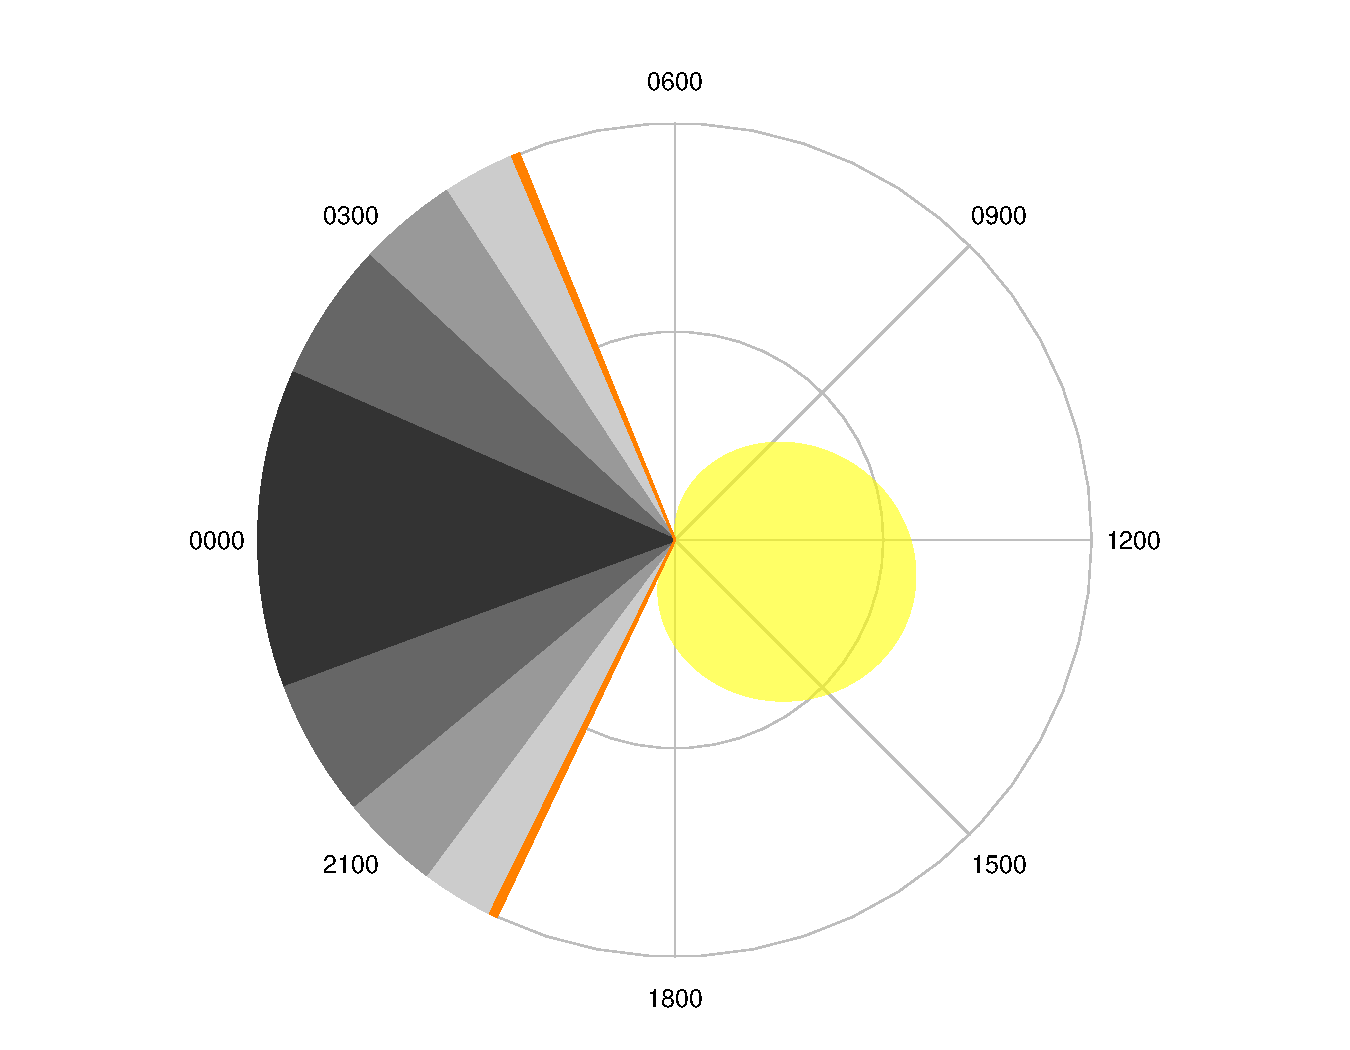
\includegraphics[width=0.9\linewidth]{_main_files/figure-latex/diel-plot-1-1} 

}

\caption{Example of a diel plot}\label{fig:diel-plot-1}
\end{figure}

\hypertarget{rotations-of-a-dielplot}{%
\subsubsection{\texorpdfstring{Rotations of a \texttt{dielPlot()}}{Rotations of a dielPlot()}}\label{rotations-of-a-dielplot}}

By default the information is plotted in the UTC timezone, so locations in other timezones will have an overall rotation.

\begin{Shaded}
\begin{Highlighting}[]
\FunctionTok{par}\NormalTok{(}\AttributeTok{mfrow=}\FunctionTok{c}\NormalTok{(}\DecValTok{1}\NormalTok{,}\DecValTok{3}\NormalTok{))}
\FunctionTok{dielPlot}\NormalTok{(}\FunctionTok{Sys.Date}\NormalTok{(), }\AttributeTok{lat=}\DecValTok{53}\NormalTok{, }\AttributeTok{lon=}\SpecialCharTok{{-}}\DecValTok{50}\NormalTok{)}
\FunctionTok{dielPlot}\NormalTok{(}\FunctionTok{Sys.Date}\NormalTok{(), }\AttributeTok{lat=}\DecValTok{53}\NormalTok{, }\AttributeTok{lon=}\SpecialCharTok{{-}}\DecValTok{0}\NormalTok{)}
\FunctionTok{dielPlot}\NormalTok{(}\FunctionTok{Sys.Date}\NormalTok{(), }\AttributeTok{lat=}\DecValTok{53}\NormalTok{, }\AttributeTok{lon=}\DecValTok{50}\NormalTok{)}
\end{Highlighting}
\end{Shaded}

\begin{figure}

{\centering 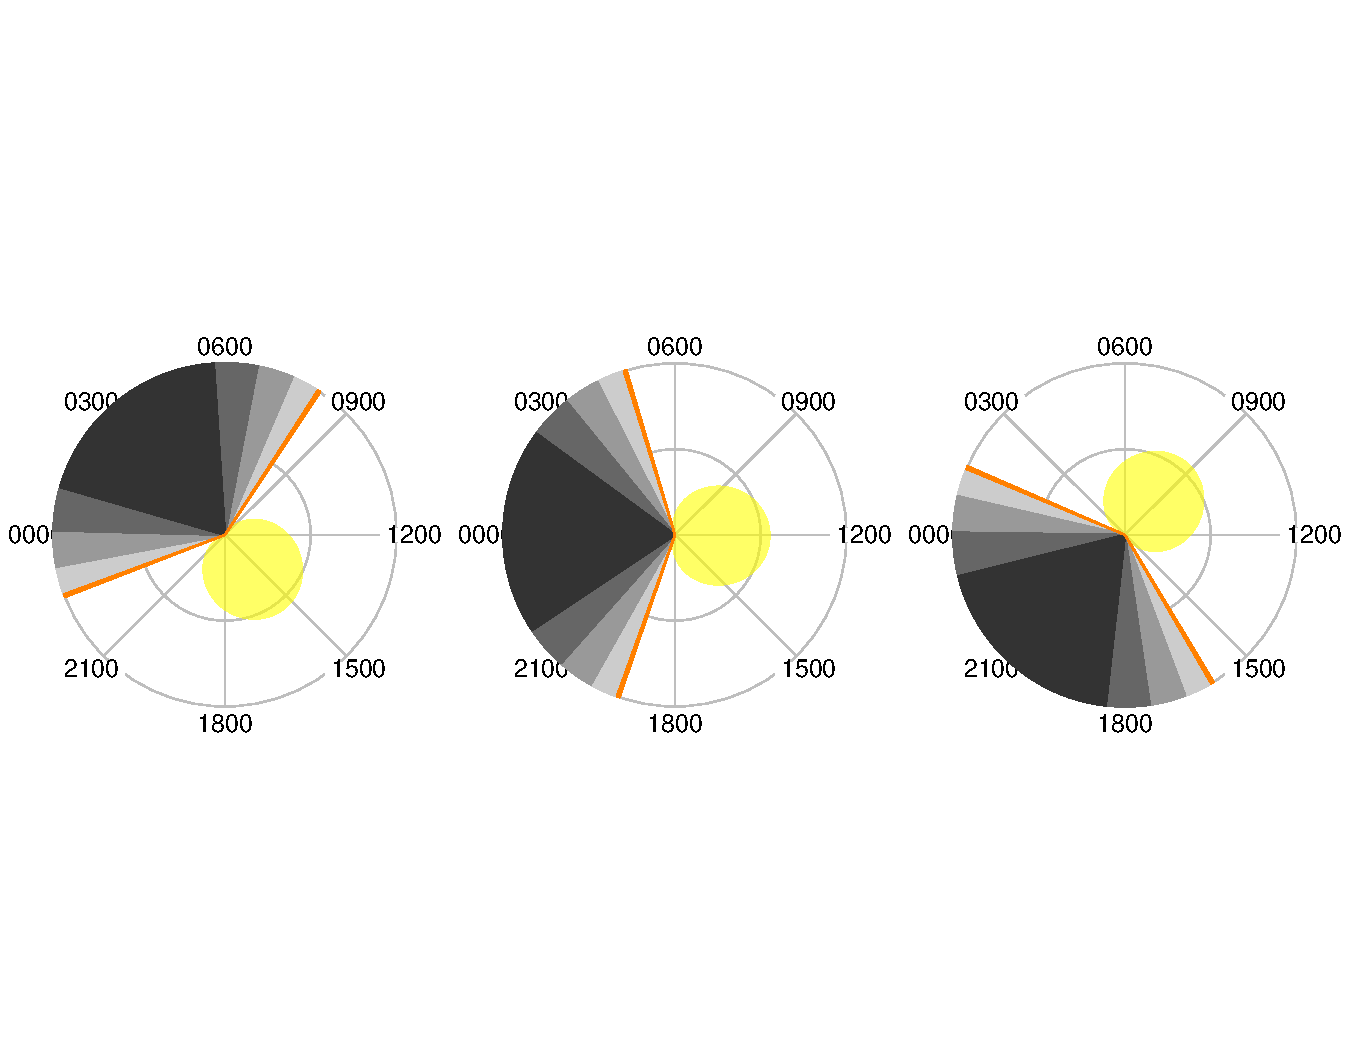
\includegraphics[width=0.9\linewidth]{_main_files/figure-latex/diel-plot-no-tz-1} 

}

\caption{Diel plots in UTC.}\label{fig:diel-plot-no-tz}
\end{figure}

Plots can be made in any timezone by using the \texttt{rot} parameter to \texttt{dielPlot()} and the \texttt{tz()} function.

\begin{Shaded}
\begin{Highlighting}[]
\FunctionTok{par}\NormalTok{(}\AttributeTok{mfrow=}\FunctionTok{c}\NormalTok{(}\DecValTok{1}\NormalTok{,}\DecValTok{3}\NormalTok{))}
\FunctionTok{dielPlot}\NormalTok{(}\FunctionTok{Sys.Date}\NormalTok{(), }\AttributeTok{lat=}\DecValTok{53}\NormalTok{, }\AttributeTok{lon=}\SpecialCharTok{{-}}\DecValTok{50}\NormalTok{, }\AttributeTok{rot=}\FunctionTok{tz}\NormalTok{(}\DecValTok{3}\NormalTok{))}
\FunctionTok{dielPlot}\NormalTok{(}\FunctionTok{Sys.Date}\NormalTok{(), }\AttributeTok{lat=}\DecValTok{53}\NormalTok{, }\AttributeTok{lon=}\SpecialCharTok{{-}}\DecValTok{0}\NormalTok{, }\AttributeTok{rot=}\FunctionTok{tz}\NormalTok{(}\DecValTok{3}\NormalTok{))}
\FunctionTok{dielPlot}\NormalTok{(}\FunctionTok{Sys.Date}\NormalTok{(), }\AttributeTok{lat=}\DecValTok{53}\NormalTok{, }\AttributeTok{lon=}\DecValTok{50}\NormalTok{, }\AttributeTok{rot=}\FunctionTok{tz}\NormalTok{(}\DecValTok{3}\NormalTok{))}
\end{Highlighting}
\end{Shaded}

\begin{figure}

{\centering 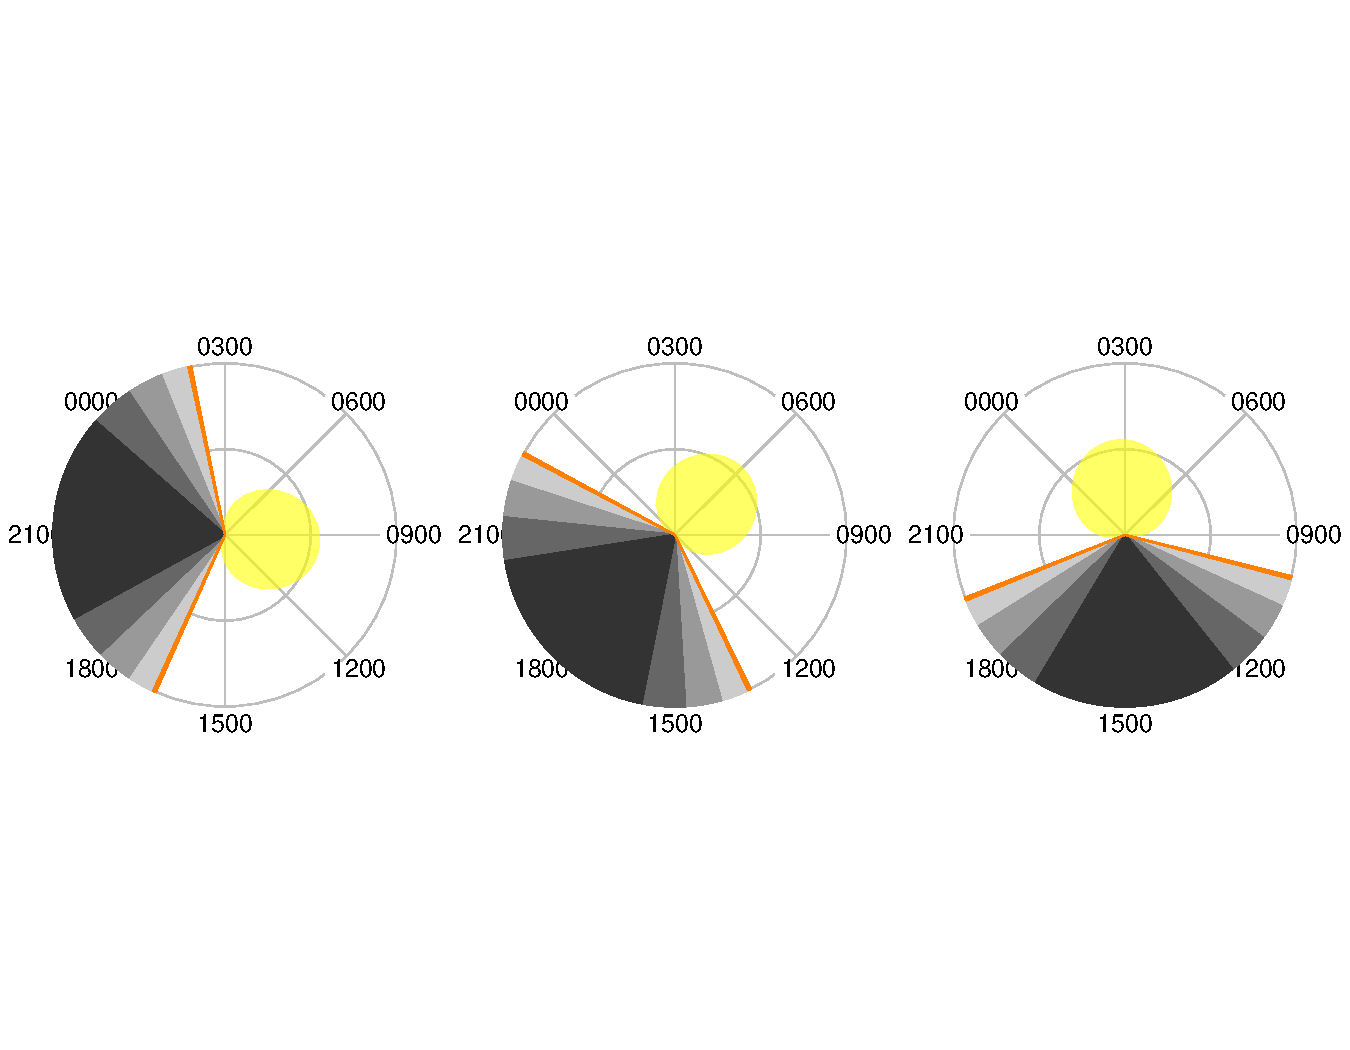
\includegraphics[width=0.9\linewidth]{_main_files/figure-latex/diel-plot-tz-1} 

}

\caption{The same diel plots in UTC +3}\label{fig:diel-plot-tz}
\end{figure}

By setting the \texttt{rot} parameter to \texttt{Solar\ Noon} it is possible to align the plots to solar noon. Notice that this rotates the plot labels.

\begin{Shaded}
\begin{Highlighting}[]
\FunctionTok{par}\NormalTok{(}\AttributeTok{mfrow=}\FunctionTok{c}\NormalTok{(}\DecValTok{1}\NormalTok{,}\DecValTok{3}\NormalTok{))}
\FunctionTok{dielPlot}\NormalTok{(}\FunctionTok{Sys.Date}\NormalTok{(), }\AttributeTok{lat=}\DecValTok{53}\NormalTok{, }\AttributeTok{lon=}\SpecialCharTok{{-}}\DecValTok{50}\NormalTok{, }\AttributeTok{rot=}\StringTok{"Solar Noon"}\NormalTok{)}
\FunctionTok{dielPlot}\NormalTok{(}\FunctionTok{Sys.Date}\NormalTok{(), }\AttributeTok{lat=}\DecValTok{53}\NormalTok{, }\AttributeTok{lon=}\SpecialCharTok{{-}}\DecValTok{0}\NormalTok{, }\AttributeTok{rot=}\StringTok{"Solar Noon"}\NormalTok{)}
\FunctionTok{dielPlot}\NormalTok{(}\FunctionTok{Sys.Date}\NormalTok{(), }\AttributeTok{lat=}\DecValTok{53}\NormalTok{, }\AttributeTok{lon=}\DecValTok{50}\NormalTok{, }\AttributeTok{rot=}\StringTok{"Solar Noon"}\NormalTok{)}
\end{Highlighting}
\end{Shaded}

\begin{figure}

{\centering 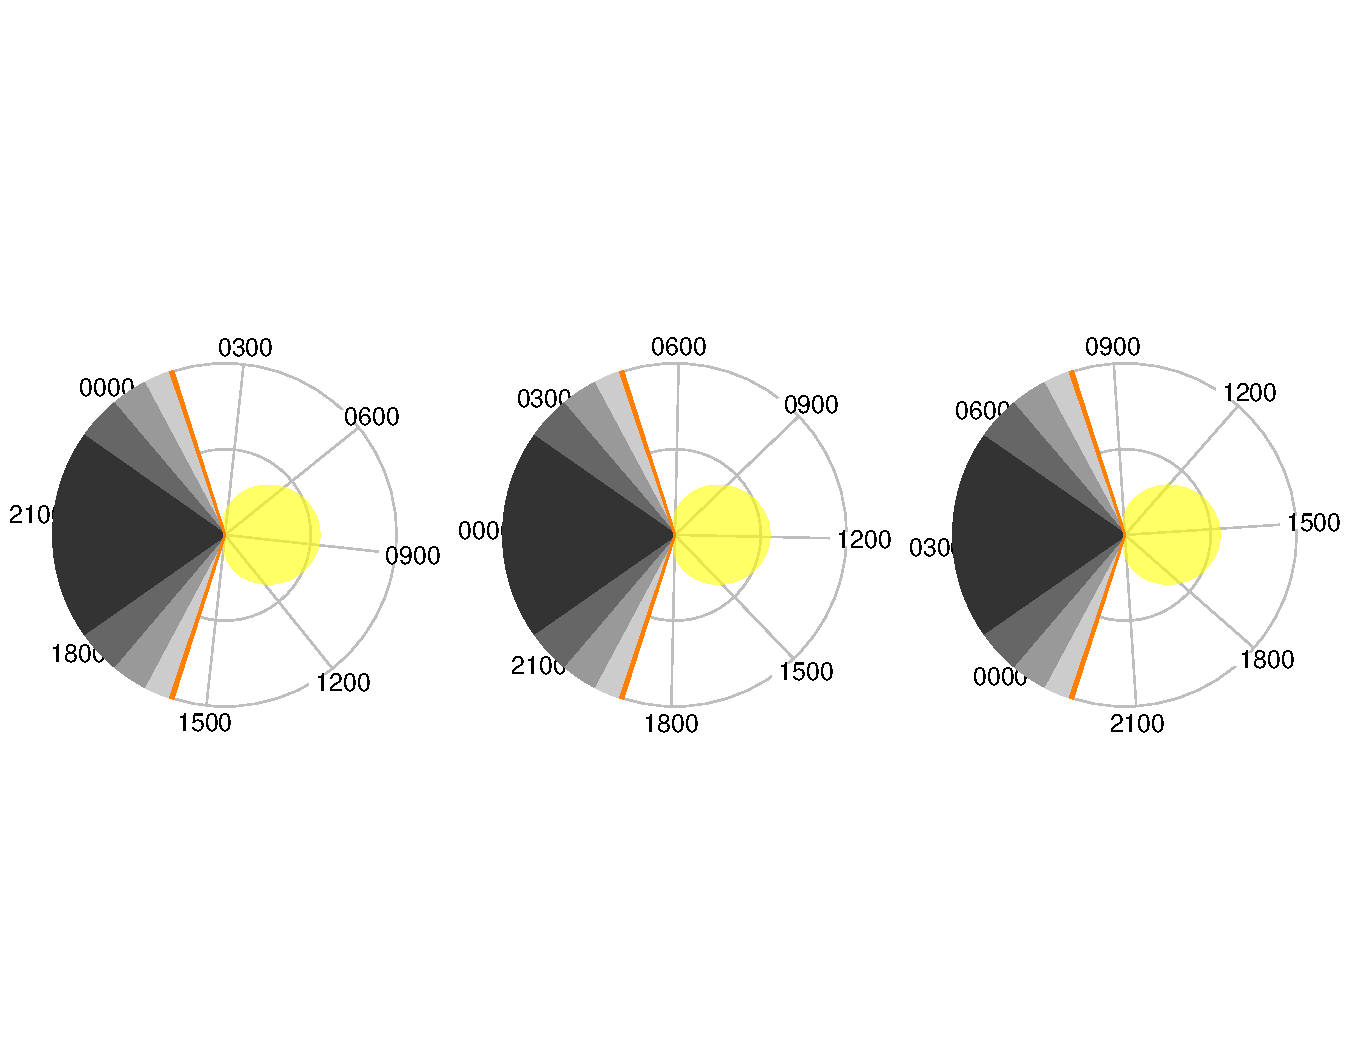
\includegraphics[width=0.9\linewidth]{_main_files/figure-latex/diel-plot-sn-1} 

}

\caption{The same diel plots aligned to solar noon}\label{fig:diel-plot-sn}
\end{figure}

\hypertarget{customising-a-dielplot}{%
\subsubsection{\texorpdfstring{Customising a \texttt{dielPlot()}}{Customising a dielPlot()}}\label{customising-a-dielplot}}

In addition to the \texttt{date}, \texttt{lat} and \texttt{lon} parameters to \texttt{dielPlot()} it is possible to make additional customisations to how the information is presented.

\textbf{Legend}

A legend can be added to the plot by setting \texttt{legend=TRUE}.

\begin{Shaded}
\begin{Highlighting}[]
\FunctionTok{dielPlot}\NormalTok{(}\StringTok{"2022{-}08{-}08"}\NormalTok{, }\AttributeTok{lat=}\DecValTok{53}\NormalTok{, }\AttributeTok{lon=}\FloatTok{0.1}\NormalTok{, }\AttributeTok{legend=}\ConstantTok{TRUE}\NormalTok{)}
\end{Highlighting}
\end{Shaded}

\begin{figure}

{\centering 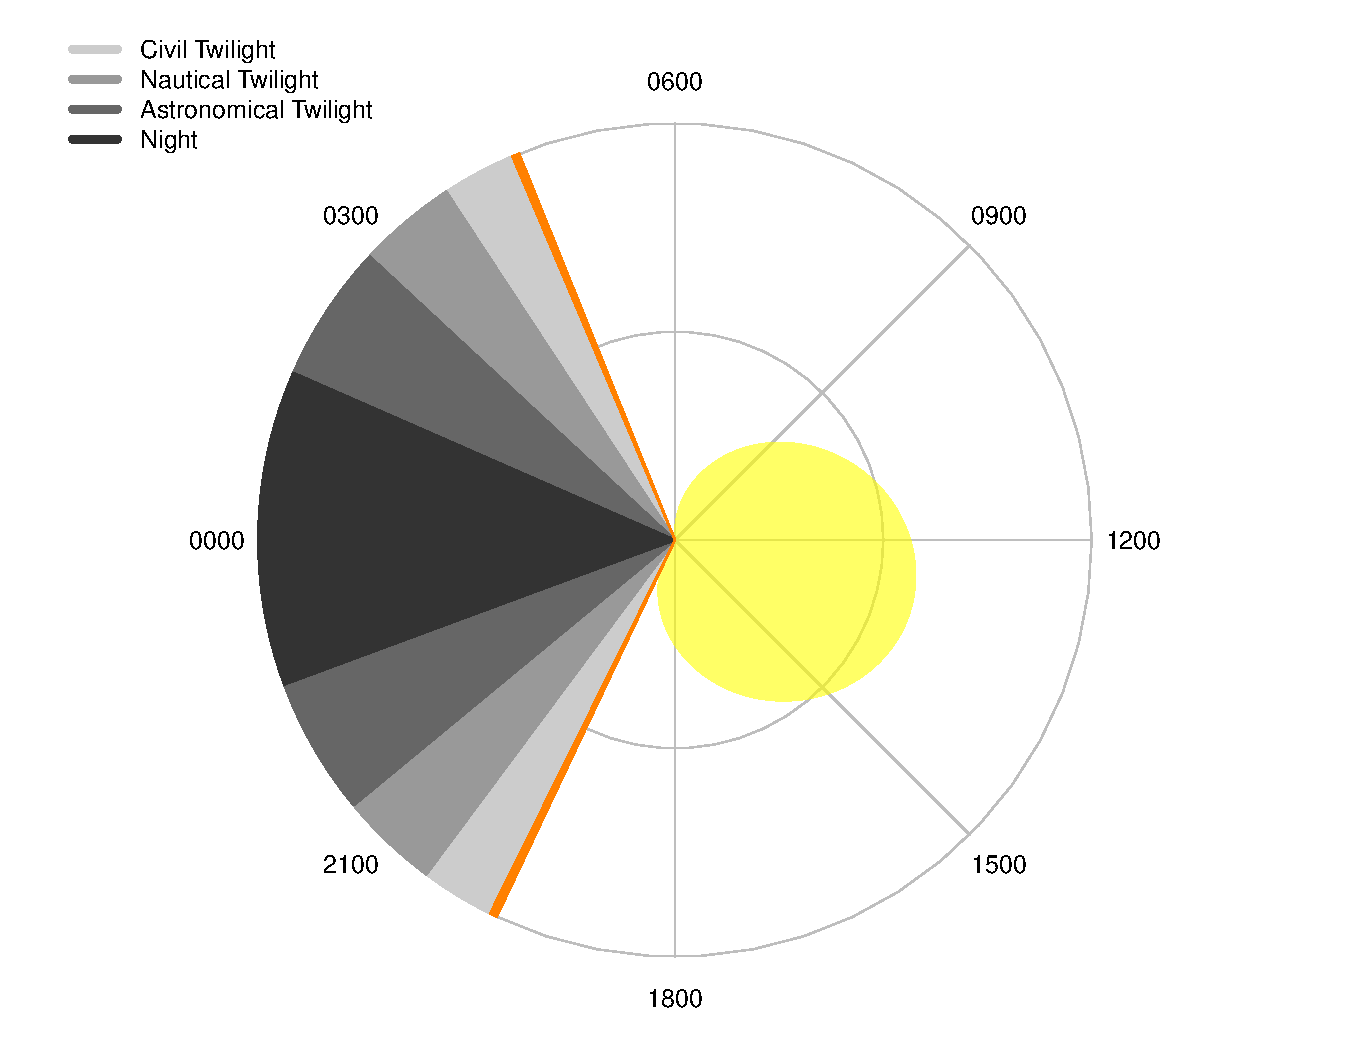
\includegraphics[width=0.9\linewidth]{_main_files/figure-latex/diel-plot-legend-1} 

}

\caption{Example adding a legend to a diel plot}\label{fig:diel-plot-legend}
\end{figure}

\textbf{Plotting Components}

The components that can be plotted are listed below. By default all are plotted except for \texttt{Solar\ Noon} and \texttt{Nadir}.

\begin{longtable}[]{@{}ll@{}}
\toprule()
Name & Notes \\
\midrule()
\endhead
Astronomical Twilight & \\
Nautical Twilight & \\
Civil Twilight & \\
Sunrise & \\
Solar Noon & The time when the sun is highest in the sky \\
Sunset & \\
Nadir & \\
\bottomrule()
\end{longtable}

The components that are plotted can be specified using the \texttt{plot} parameter.

\begin{Shaded}
\begin{Highlighting}[]
\NormalTok{components }\OtherTok{\textless{}{-}} \FunctionTok{c}\NormalTok{(}\StringTok{"Sunrise"}\NormalTok{, }\StringTok{"Sunset"}\NormalTok{, }\StringTok{"Solar Noon"}\NormalTok{, }\StringTok{"Nadir"}\NormalTok{)}
\FunctionTok{dielPlot}\NormalTok{(}\StringTok{"2022{-}08{-}08"}\NormalTok{, }\AttributeTok{lat=}\DecValTok{53}\NormalTok{, }\AttributeTok{lon=}\FloatTok{0.1}\NormalTok{, }\AttributeTok{plot=}\NormalTok{components)}
\end{Highlighting}
\end{Shaded}

\begin{figure}

{\centering 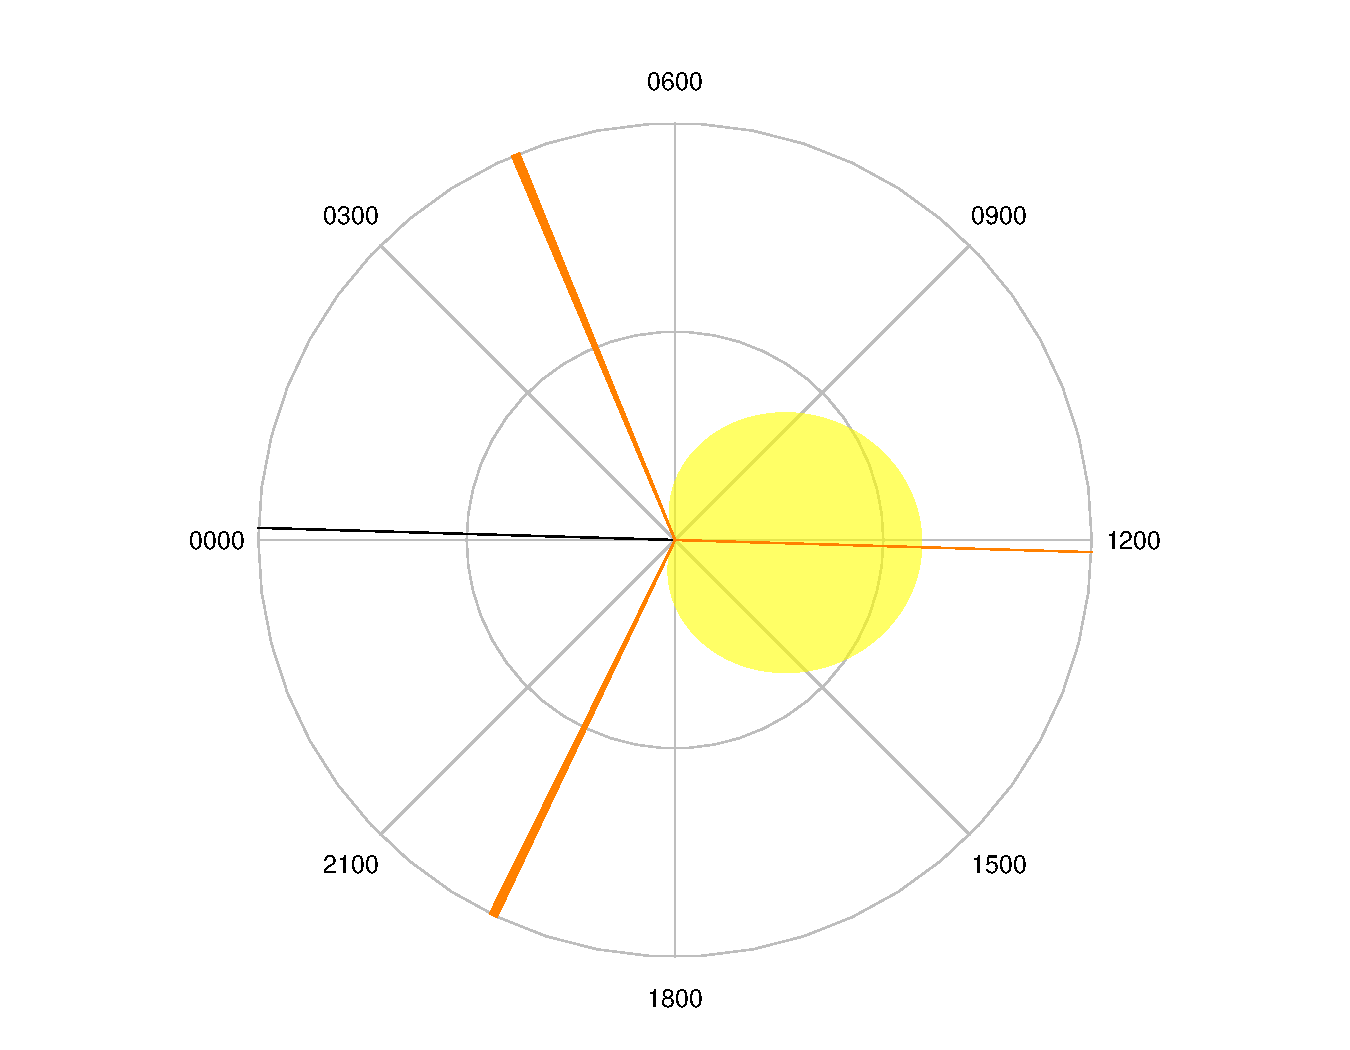
\includegraphics[width=0.9\linewidth]{_main_files/figure-latex/diel-plot-components-1} 

}

\caption{Selecting the components to plot}\label{fig:diel-plot-components}
\end{figure}

\hypertarget{yearly-cycles}{%
\section{Yearly Cycles}\label{yearly-cycles}}

The \texttt{yearlyPlot()} function from the SonicScrewdriver package shows daylight changes throughout a year. It behaves in a very similar fashion to \texttt{dielPlot} but takes a single year rather a date as input.

\begin{Shaded}
\begin{Highlighting}[]
\FunctionTok{yearlyPlot}\NormalTok{(}\DecValTok{2022}\NormalTok{, }\AttributeTok{lat=}\DecValTok{53}\NormalTok{, }\AttributeTok{lon=}\FloatTok{0.1}\NormalTok{)}
\end{Highlighting}
\end{Shaded}

\begin{figure}

{\centering 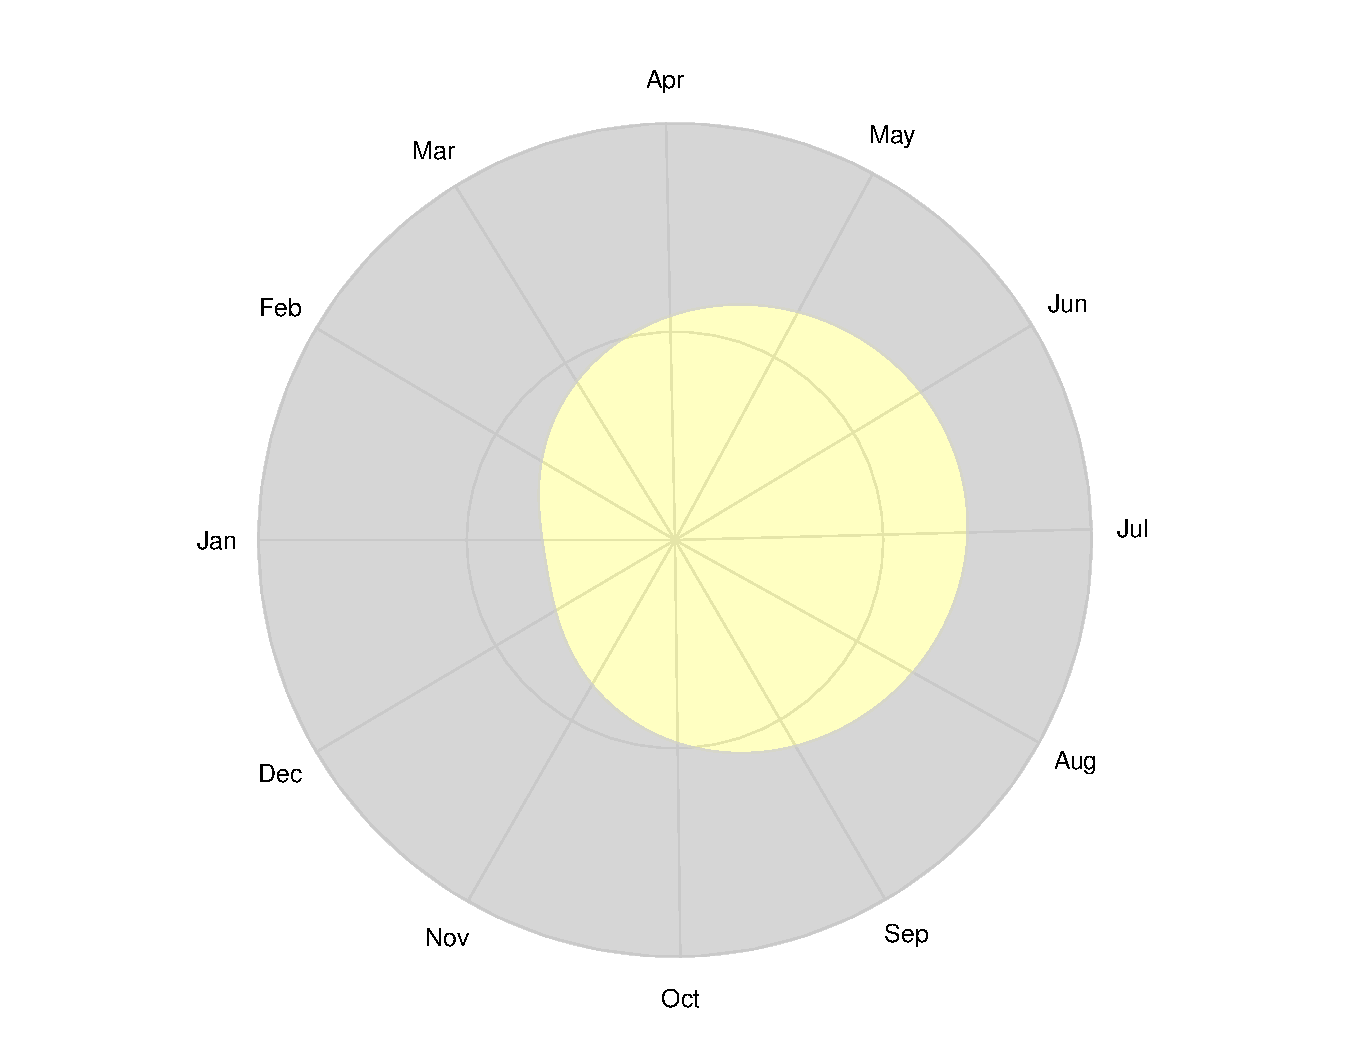
\includegraphics[width=0.9\linewidth]{_main_files/figure-latex/yearly-plot-1-1} 

}

\caption{Example of a yearly plot}\label{fig:yearly-plot-1}
\end{figure}

\hypertarget{lunar-cycles}{%
\section{Lunar Cycles}\label{lunar-cycles}}

\hypertarget{core-and-ring-plots}{%
\section{Core and ring plots}\label{core-and-ring-plots}}

These visualisations for cyclical data plot their information onto a circle with radius of two units. It is possible to limit the plot either to the centre of the circle (a `core' plot) or to the edge (a `ring plot'). These alternative forms may be more useful when these plots are used to visualise addition variables (\ref{adding-to-cyclical}).

\begin{Shaded}
\begin{Highlighting}[]
\FunctionTok{dielPlot}\NormalTok{(}\StringTok{"2022{-}08{-}08"}\NormalTok{, }\AttributeTok{lat=}\DecValTok{53}\NormalTok{, }\AttributeTok{lon=}\FloatTok{0.1}\NormalTok{, }\AttributeTok{limits=}\FunctionTok{c}\NormalTok{(}\DecValTok{0}\NormalTok{,}\DecValTok{1}\NormalTok{))}
\end{Highlighting}
\end{Shaded}

\begin{figure}

{\centering 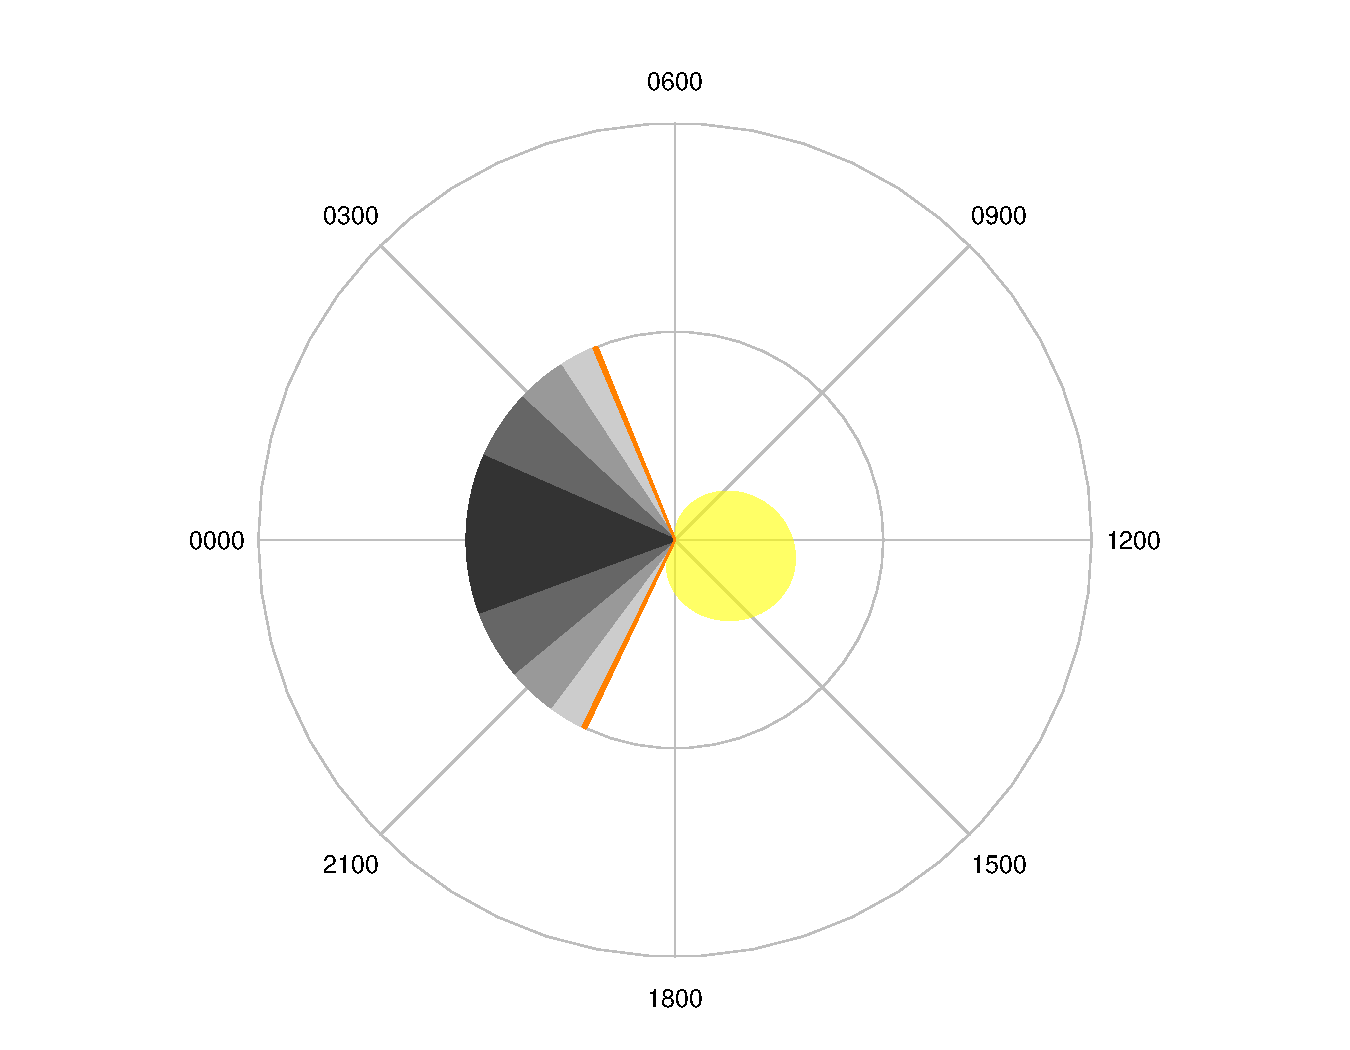
\includegraphics[width=0.9\linewidth]{_main_files/figure-latex/diel-plot-core-1} 

}

\caption{A 'core' diel plot.}\label{fig:diel-plot-core}
\end{figure}

\begin{Shaded}
\begin{Highlighting}[]
\FunctionTok{dielPlot}\NormalTok{(}\StringTok{"2022{-}08{-}08"}\NormalTok{, }\AttributeTok{lat=}\DecValTok{53}\NormalTok{, }\AttributeTok{lon=}\FloatTok{0.1}\NormalTok{, }\AttributeTok{limits=}\FunctionTok{c}\NormalTok{(}\DecValTok{1}\NormalTok{,}\DecValTok{2}\NormalTok{))}
\end{Highlighting}
\end{Shaded}

\begin{figure}

{\centering 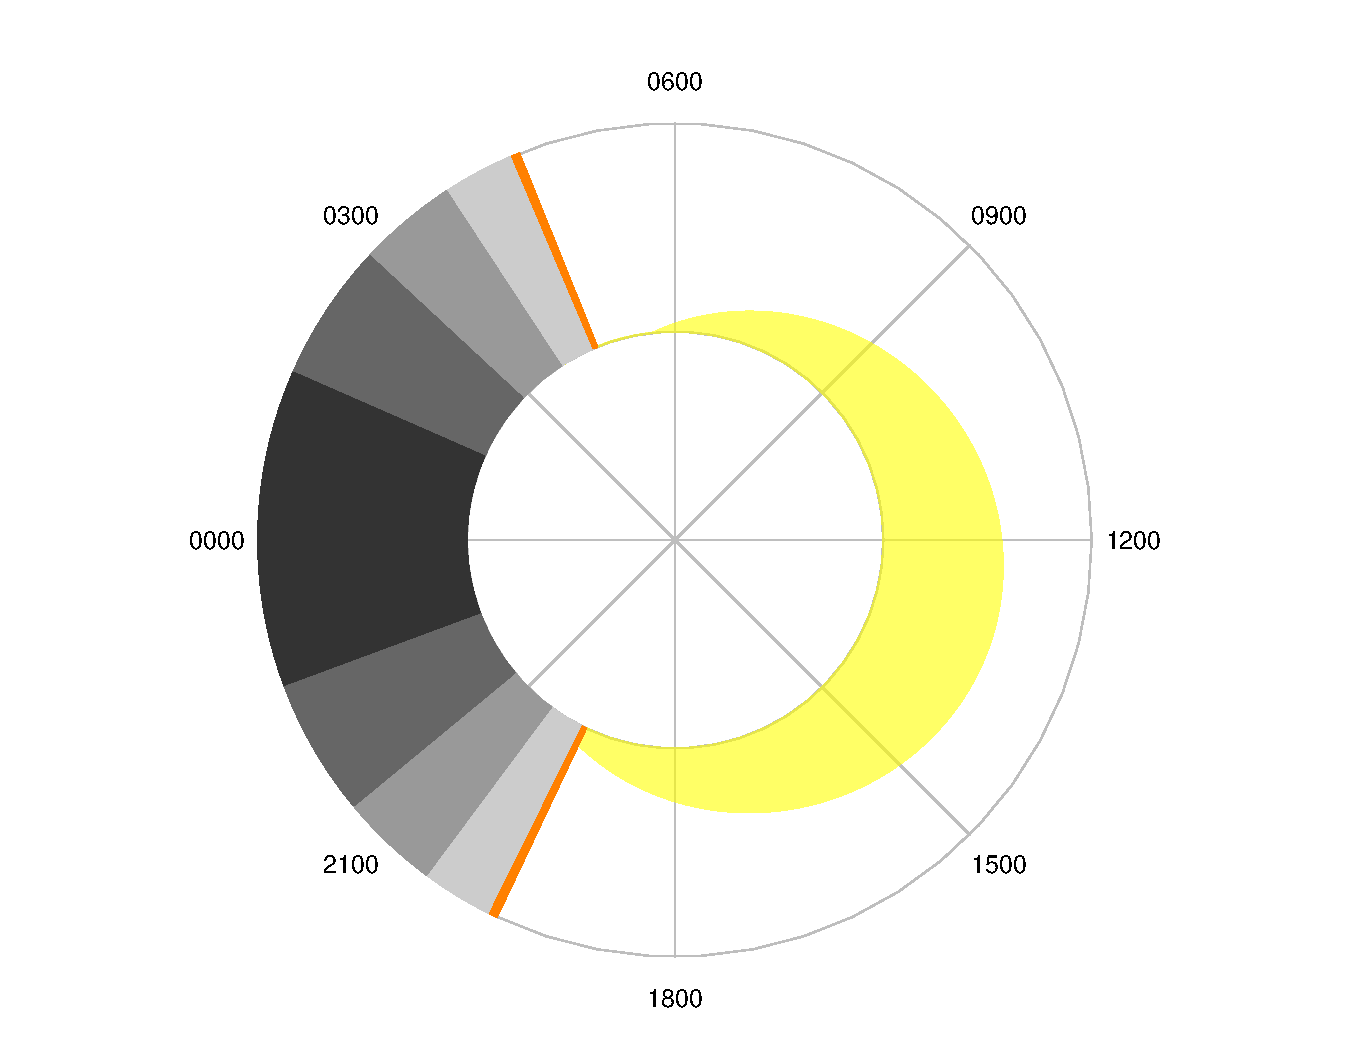
\includegraphics[width=0.9\linewidth]{_main_files/figure-latex/diel-plot-ring-1} 

}

\caption{A 'ring' diel plot.}\label{fig:diel-plot-ring}
\end{figure}

\hypertarget{behind-the-scenes}{%
\section{Behind the scenes}\label{behind-the-scenes}}

\hypertarget{radialpolygon}{%
\subsection{\texorpdfstring{\texttt{radialPolygon()}}{radialPolygon()}}\label{radialpolygon}}

The majority of the plotting performed for cyclical plots in \texttt{SonicScrewdriver} is performed by the \texttt{radialPolygon()} function. This function can be used to plot sectors, annuli, horizon plots and irregular polygons. It is used by the plotting functions such as \texttt{dielPlot()} as well as helper functions such as \texttt{dielRings()} to add data to cyclical plots.

For simple use cases, knowledge of the operation of \texttt{radialPolygon()} may not be needed. A number of helper functions cover the most common uses. However, an understanding of how this function works will allow for far greater customisation of cyclical plots than would otherwise be possible.

\begin{figure}

{\centering 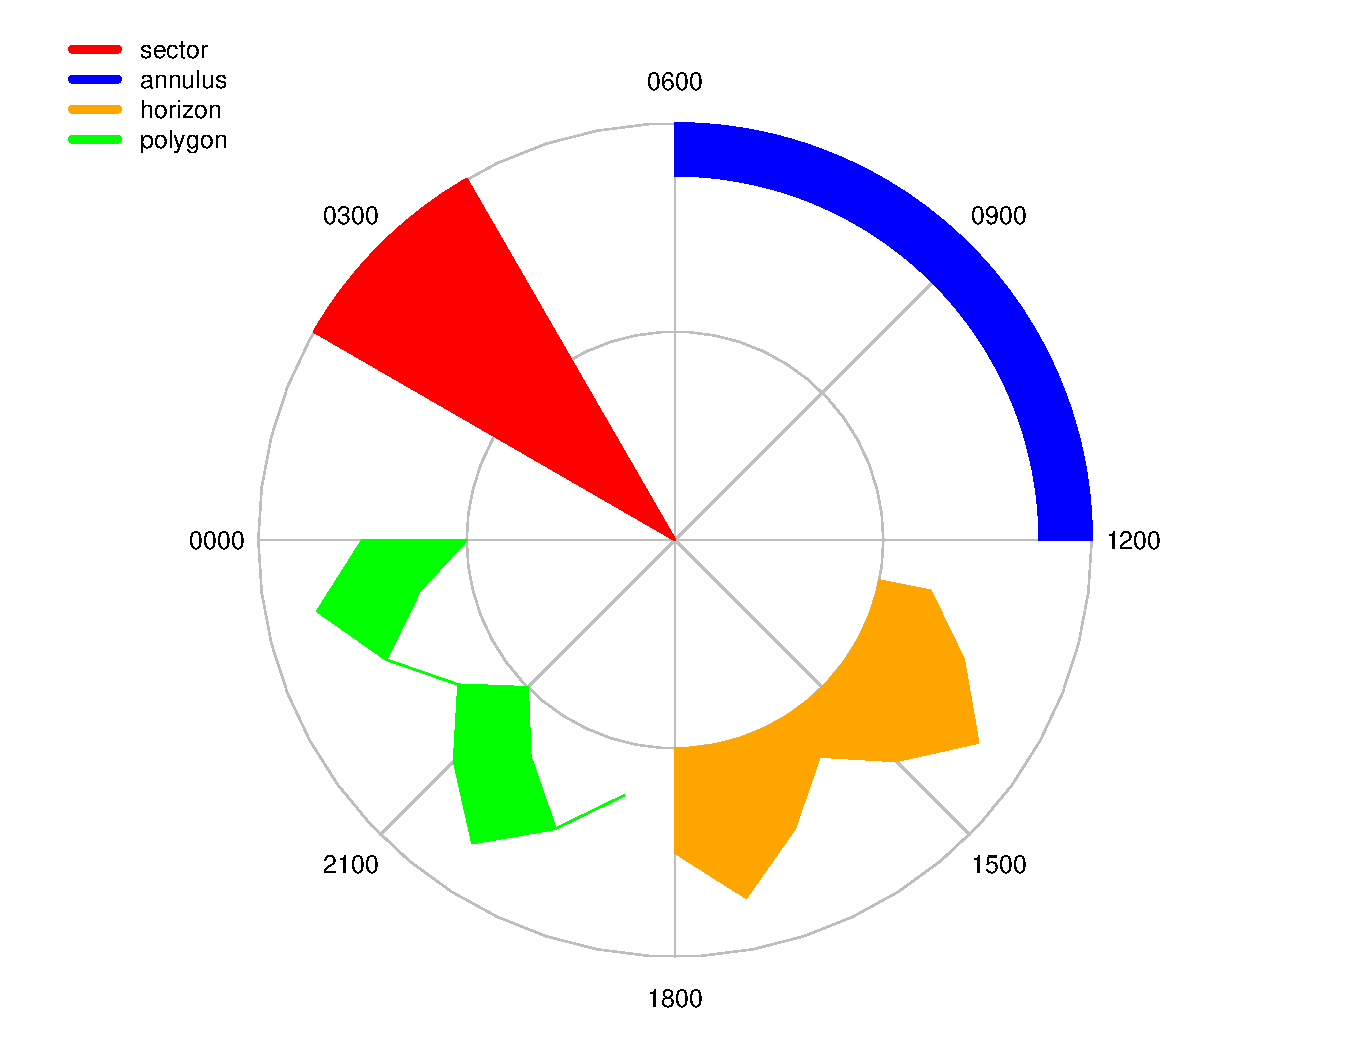
\includegraphics[width=0.9\linewidth]{_main_files/figure-latex/radialPolygon-types-1} 

}

\caption{Types of radial polygon plot}\label{fig:radialPolygon-types}
\end{figure}

The various types of plots are created by changing the angle and radius parameters to \texttt{radialPolygon().}

\begin{Shaded}
\begin{Highlighting}[]
\FunctionTok{radialPolygon}\NormalTok{(angle1, angle2, radius1, radius2, col)}
\end{Highlighting}
\end{Shaded}

\hypertarget{orientation}{%
\subsubsection{Orientation}\label{orientation}}

Unlike traditional polar plots, diel and yearly plots start their periods on the left hand horizontal, and proceed clockwise. This orientation is assumed by \texttt{radialPolygon()}, although it may be modified (e.g.~the parameters \texttt{reverse=FALSE} and \texttt{rot=0} will plot using the standard conventions for polar coordinate systems.)

\hypertarget{sectors}{%
\subsubsection{Sectors}\label{sectors}}

A sector is a section of a circle defined by two radii and an arc between them. Sectors are used widely in the default settings of \texttt{dielPlot()} to plot the times of night and twilight.

\begin{Shaded}
\begin{Highlighting}[]
\FunctionTok{emptyDiel}\NormalTok{()}
\FunctionTok{radialPolygon}\NormalTok{(pi}\SpecialCharTok{/}\DecValTok{6}\NormalTok{, }\DecValTok{2}\SpecialCharTok{*}\NormalTok{pi}\SpecialCharTok{/}\DecValTok{3}\NormalTok{, }\DecValTok{0}\NormalTok{, }\DecValTok{2}\NormalTok{, }\AttributeTok{col=}\StringTok{"red"}\NormalTok{)}
\end{Highlighting}
\end{Shaded}

\begin{figure}

{\centering 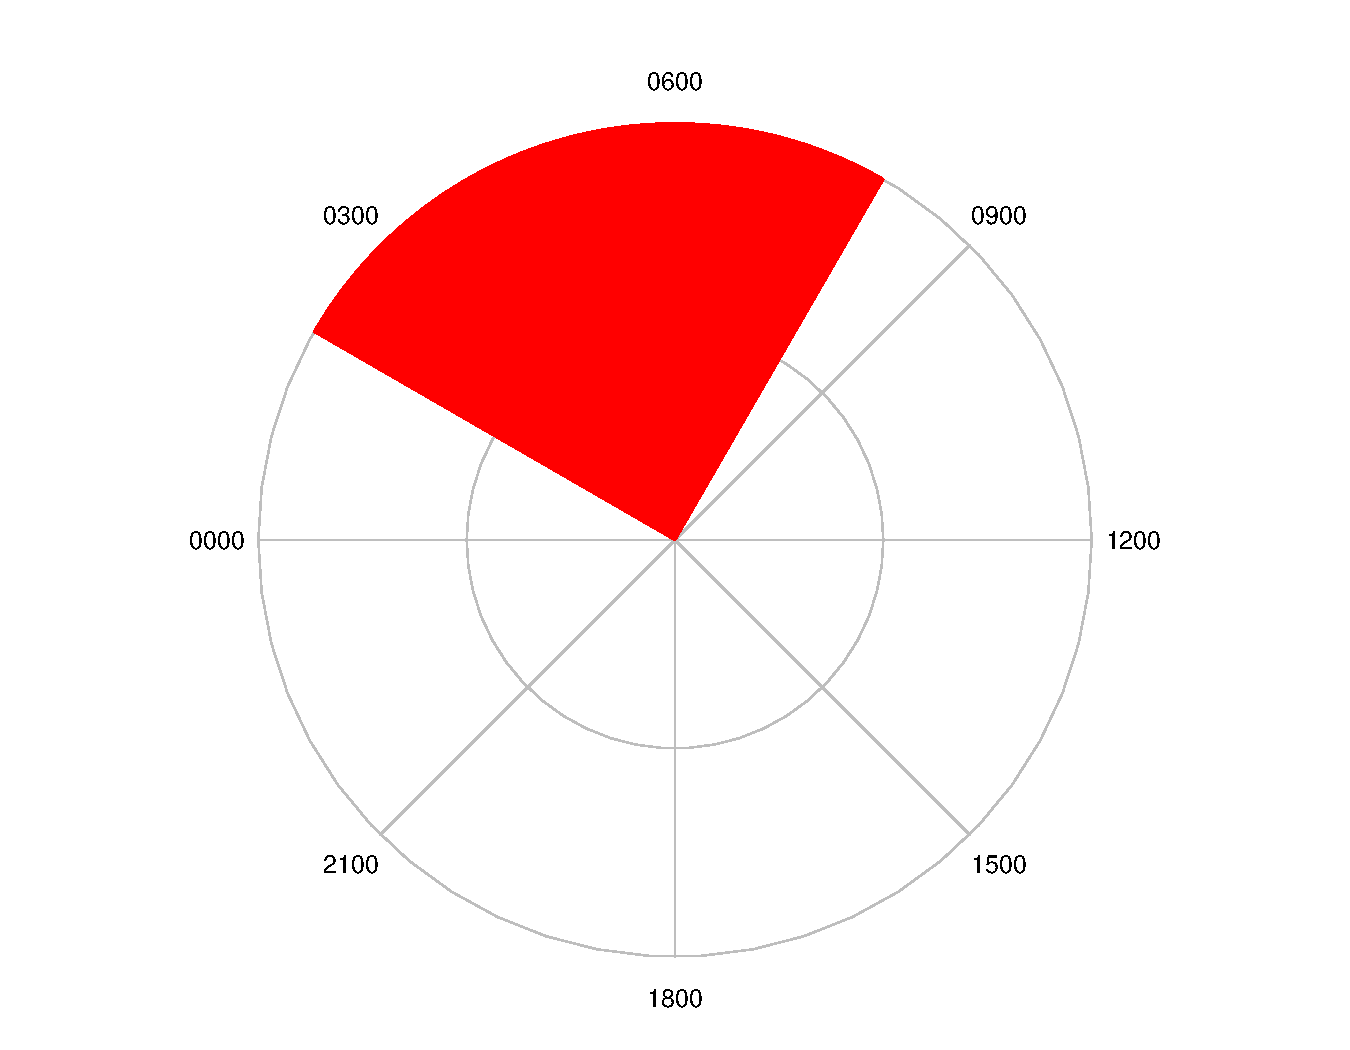
\includegraphics[width=0.9\linewidth]{_main_files/figure-latex/radialPolygon-sector-1} 

}

\caption{Plotting a sector}\label{fig:radialPolygon-sector}
\end{figure}

Reversing the angle arguments allows the complementary sector to be drawn.

\begin{Shaded}
\begin{Highlighting}[]
\FunctionTok{emptyDiel}\NormalTok{()}
\FunctionTok{radialPolygon}\NormalTok{(}\DecValTok{2}\SpecialCharTok{*}\NormalTok{pi}\SpecialCharTok{/}\DecValTok{3}\NormalTok{, pi}\SpecialCharTok{/}\DecValTok{6}\NormalTok{, }\DecValTok{0}\NormalTok{, }\DecValTok{2}\NormalTok{, }\AttributeTok{col=}\StringTok{"blue"}\NormalTok{)}
\end{Highlighting}
\end{Shaded}

\begin{figure}

{\centering 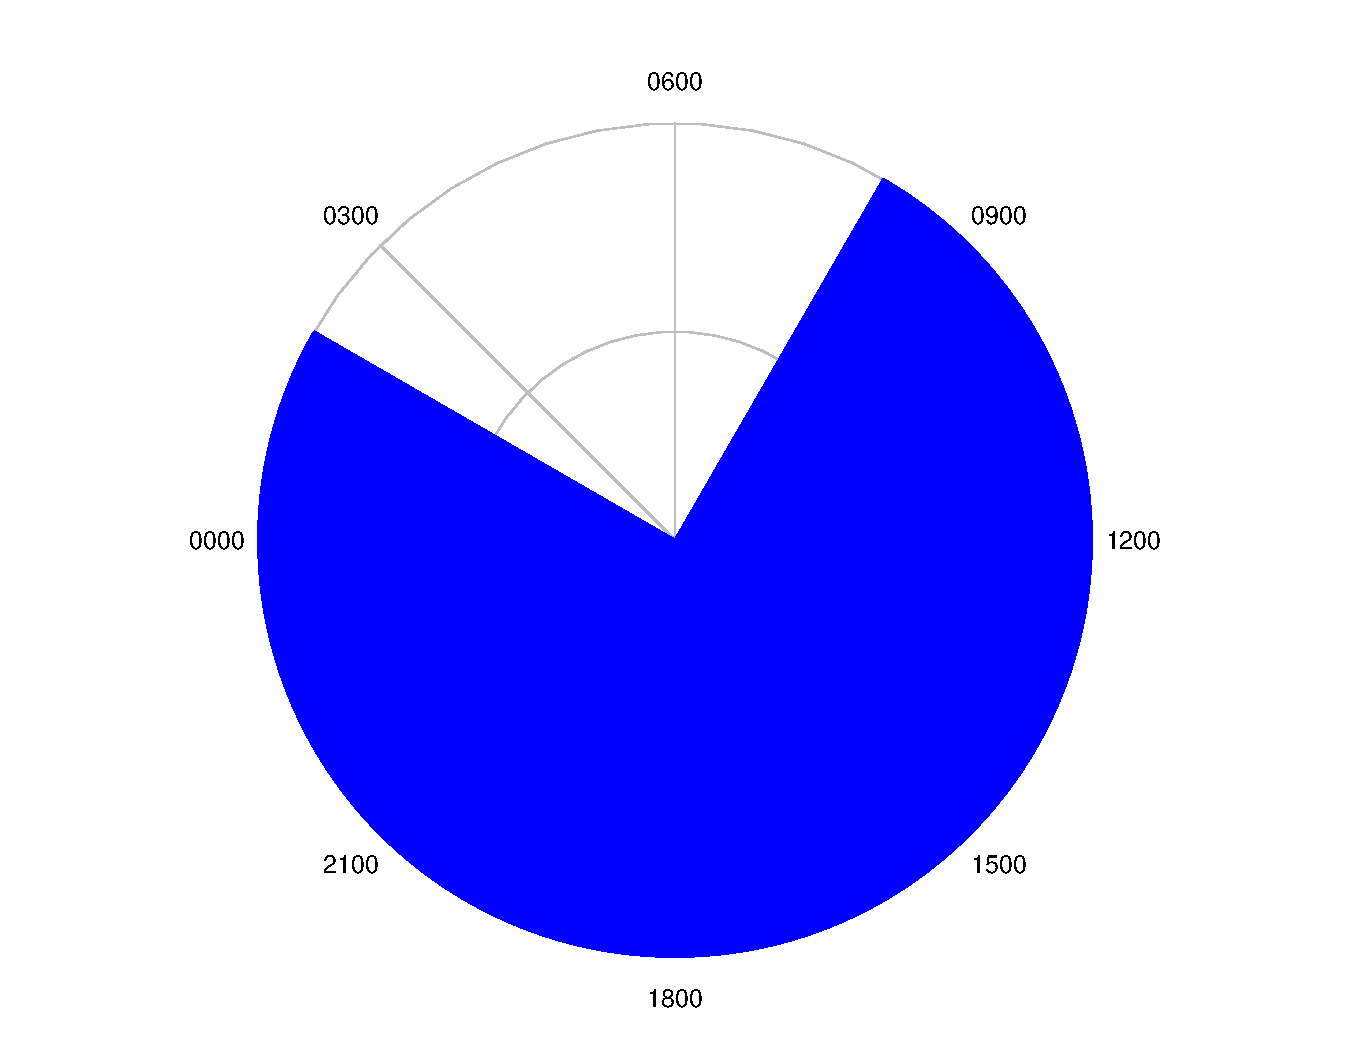
\includegraphics[width=0.9\linewidth]{_main_files/figure-latex/radialPolygon-sector2-1} 

}

\caption{Plotting a sector}\label{fig:radialPolygon-sector2}
\end{figure}

\hypertarget{annuli}{%
\subsubsection{Annuli}\label{annuli}}

An annulus is the region between two concentric circles. Annuli and annular sectors are generated by \texttt{radialPolygon()} when the parameter \texttt{radius} is greater than zero.

\begin{Shaded}
\begin{Highlighting}[]
\FunctionTok{emptyDiel}\NormalTok{()}
\FunctionTok{radialPolygon}\NormalTok{(}\DecValTok{0}\NormalTok{, }\DecValTok{2}\SpecialCharTok{*}\NormalTok{pi, }\FloatTok{1.75}\NormalTok{, }\DecValTok{2}\NormalTok{, }\AttributeTok{col=}\StringTok{"blue"}\NormalTok{)}
\FunctionTok{radialPolygon}\NormalTok{(pi, }\DecValTok{4}\SpecialCharTok{*}\NormalTok{pi}\SpecialCharTok{/}\DecValTok{3}\NormalTok{, }\DecValTok{1}\NormalTok{, }\FloatTok{1.5}\NormalTok{, }\AttributeTok{col=}\StringTok{"red"}\NormalTok{)}
\FunctionTok{legend}\NormalTok{(}
  \SpecialCharTok{{-}}\DecValTok{3}\NormalTok{,}\FloatTok{2.5}\NormalTok{,}
  \FunctionTok{c}\NormalTok{(}\StringTok{"annulus"}\NormalTok{, }\StringTok{"annuluar sector"}\NormalTok{),}
  \AttributeTok{col=}\FunctionTok{c}\NormalTok{(}\StringTok{"blue"}\NormalTok{, }\StringTok{"red"}\NormalTok{),}
  \AttributeTok{lty=}\DecValTok{1}\NormalTok{,}
  \AttributeTok{lwd=}\DecValTok{5}\NormalTok{,}
  \AttributeTok{bty =} \StringTok{"n"}\NormalTok{,}
  \AttributeTok{cex =} \DecValTok{1}\NormalTok{)}
\end{Highlighting}
\end{Shaded}

\begin{figure}

{\centering 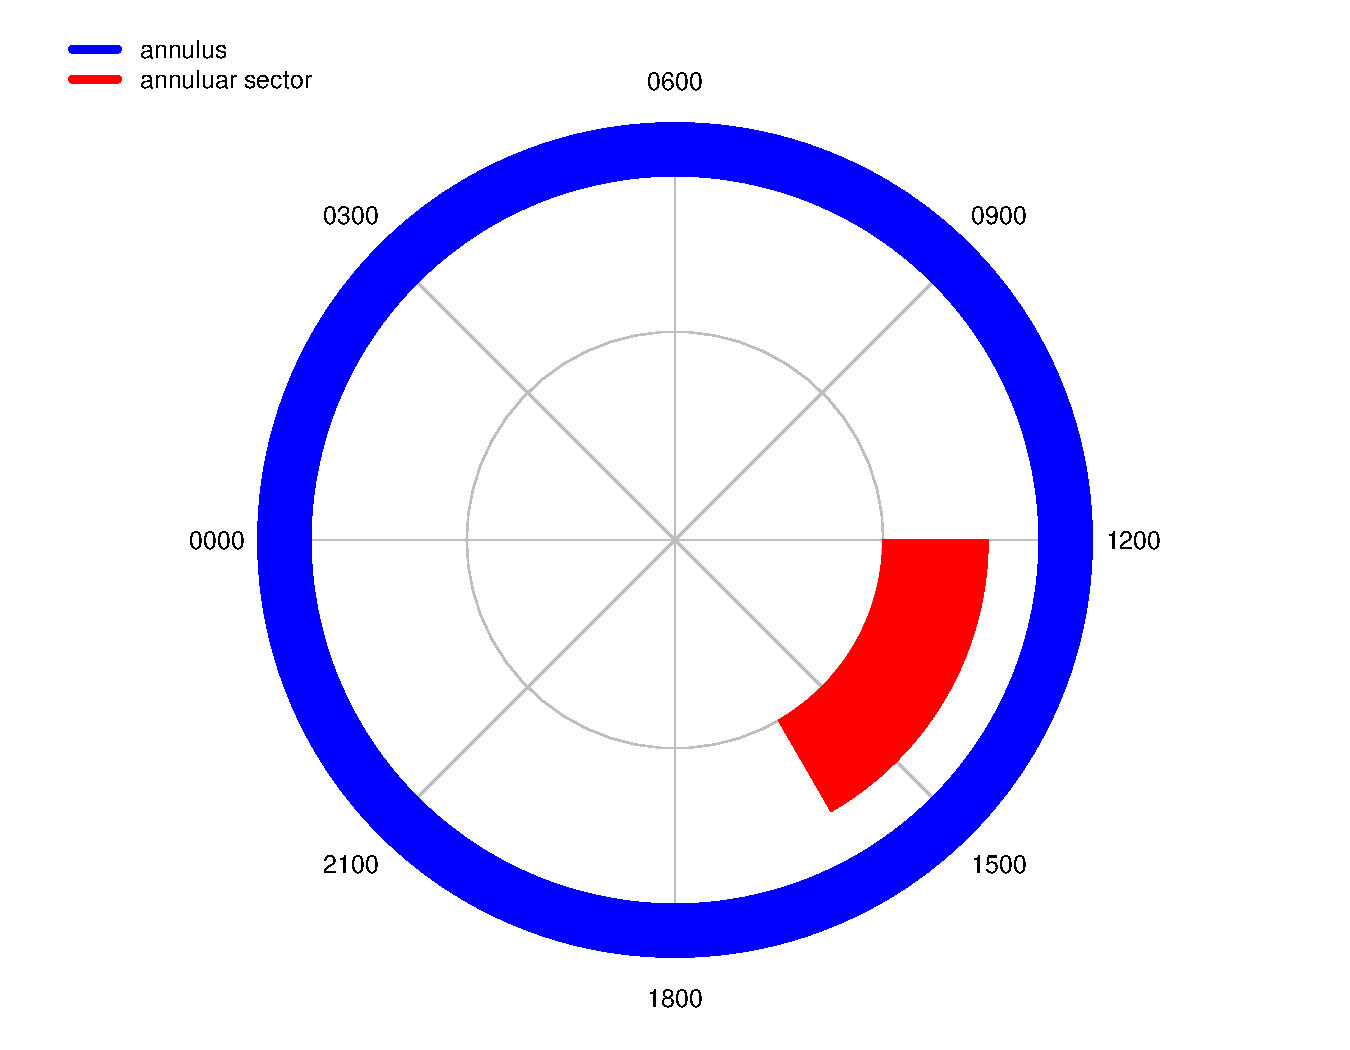
\includegraphics[width=0.9\linewidth]{_main_files/figure-latex/radialPolygon-annuli-1} 

}

\caption{Plotting an annulus and an annular sector}\label{fig:radialPolygon-annuli}
\end{figure}

\hypertarget{horizons}{%
\subsubsection{Horizons}\label{horizons}}

Horizons have one circular edge, and one that represents data, they are named as they often resemble a landscape or cityscape horizon. The example below uses a generated sine pattern to form the data edge.

\begin{Shaded}
\begin{Highlighting}[]
\FunctionTok{library}\NormalTok{(tuneR)}

\NormalTok{angles }\OtherTok{\textless{}{-}}\NormalTok{ (}\DecValTok{0}\SpecialCharTok{:}\DecValTok{200}\NormalTok{)}\SpecialCharTok{*}\NormalTok{pi}\SpecialCharTok{/}\DecValTok{200} \SpecialCharTok{+}\NormalTok{ pi}\SpecialCharTok{/}\DecValTok{2}
\NormalTok{values }\OtherTok{\textless{}{-}} \FloatTok{0.05}\SpecialCharTok{*}\FunctionTok{sine}\NormalTok{(}\DecValTok{10}\NormalTok{, }\AttributeTok{samp.rate=}\DecValTok{201}\NormalTok{)}\SpecialCharTok{@}\NormalTok{left}

\FunctionTok{emptyDiel}\NormalTok{()}
\FunctionTok{radialPolygon}\NormalTok{(}\ConstantTok{NA}\NormalTok{,angles,}\FloatTok{0.5}\NormalTok{,}\DecValTok{1}\SpecialCharTok{+}\NormalTok{values)}
\end{Highlighting}
\end{Shaded}

\begin{figure}

{\centering 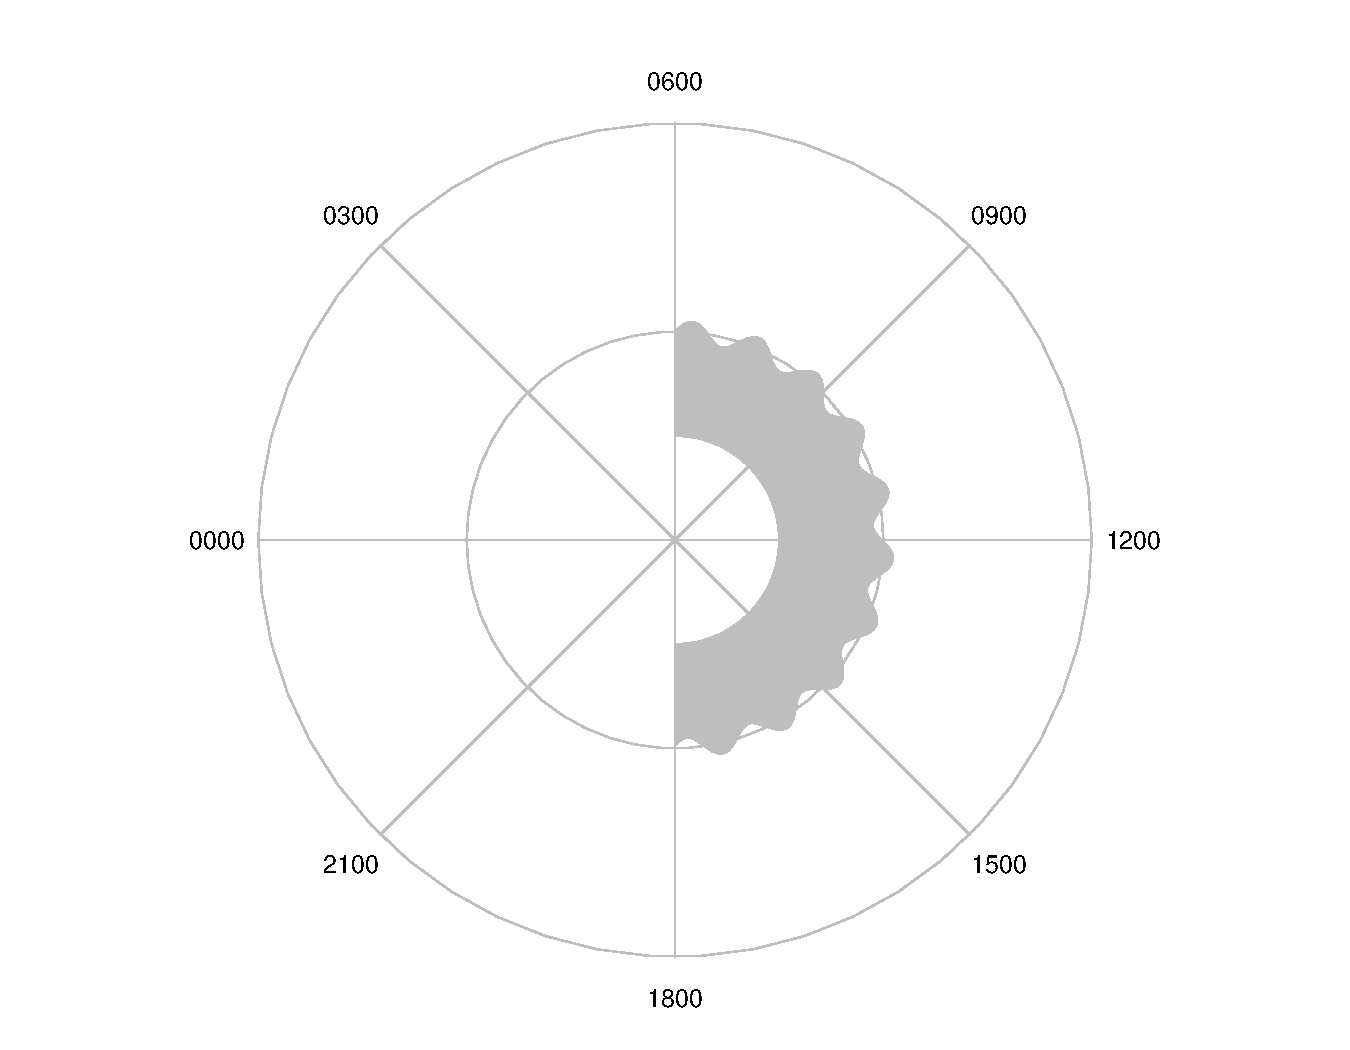
\includegraphics[width=0.9\linewidth]{_main_files/figure-latex/radialPolygon-horizon-1} 

}

\caption{Plotting a horizon polygon.}\label{fig:radialPolygon-horizon}
\end{figure}

Setting the first angle parameter to \texttt{NA} uses the range of the second to calculate the inner edge.

The inner edge can be used to show data by swapping the order of the angle and radius parameters.

\begin{Shaded}
\begin{Highlighting}[]
\FunctionTok{library}\NormalTok{(tuneR)}

\NormalTok{angles }\OtherTok{\textless{}{-}}\NormalTok{ (}\DecValTok{0}\SpecialCharTok{:}\DecValTok{200}\NormalTok{)}\SpecialCharTok{*}\NormalTok{pi}\SpecialCharTok{/}\DecValTok{200} \SpecialCharTok{+}\NormalTok{ pi}\SpecialCharTok{/}\DecValTok{2}
\NormalTok{values }\OtherTok{\textless{}{-}} \FloatTok{0.05}\SpecialCharTok{*}\FunctionTok{sine}\NormalTok{(}\DecValTok{10}\NormalTok{, }\AttributeTok{samp.rate=}\DecValTok{201}\NormalTok{)}\SpecialCharTok{@}\NormalTok{left}

\FunctionTok{emptyDiel}\NormalTok{()}
\FunctionTok{radialPolygon}\NormalTok{(angles,}\ConstantTok{NA}\NormalTok{,}\DecValTok{1}\SpecialCharTok{+}\NormalTok{values,}\DecValTok{2}\NormalTok{)}
\end{Highlighting}
\end{Shaded}

\begin{figure}

{\centering 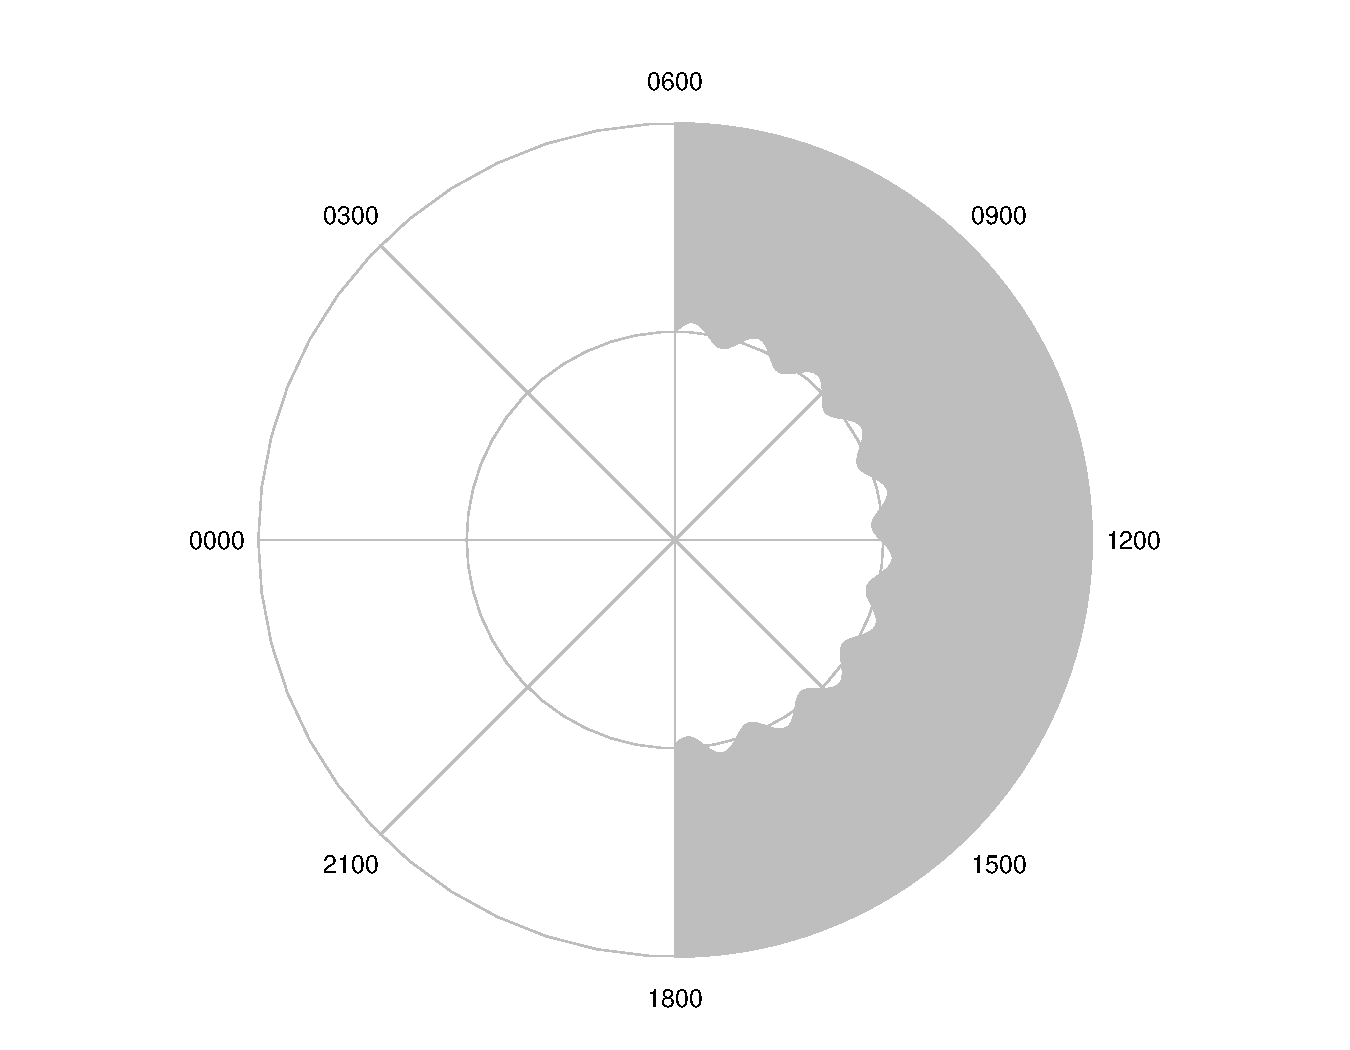
\includegraphics[width=0.9\linewidth]{_main_files/figure-latex/radialPolygon-horizon2-1} 

}

\caption{Plotting a horizon polygon.}\label{fig:radialPolygon-horizon2}
\end{figure}

The \texttt{yearlyPlot()} function uses two horizon plots, with a shared data edge.

\hypertarget{polygons}{%
\subsubsection{Polygons}\label{polygons}}

\hypertarget{empty-plots}{%
\section{Empty plots}\label{empty-plots}}

The uses of daily and yearly plots extend beyond linking data to earthly cycles. The following functions provide the basic coordinate system without any data plotted (these functions are used intenally by \texttt{dielPlot()} and \texttt{yearlyPlot()} to establish their coordinate system).

\hypertarget{emptydiel}{%
\subsection{\texorpdfstring{\texttt{emptyDiel()}}{emptyDiel()}}\label{emptydiel}}

\begin{Shaded}
\begin{Highlighting}[]
\FunctionTok{emptyDiel}\NormalTok{()}
\end{Highlighting}
\end{Shaded}

\begin{figure}

{\centering 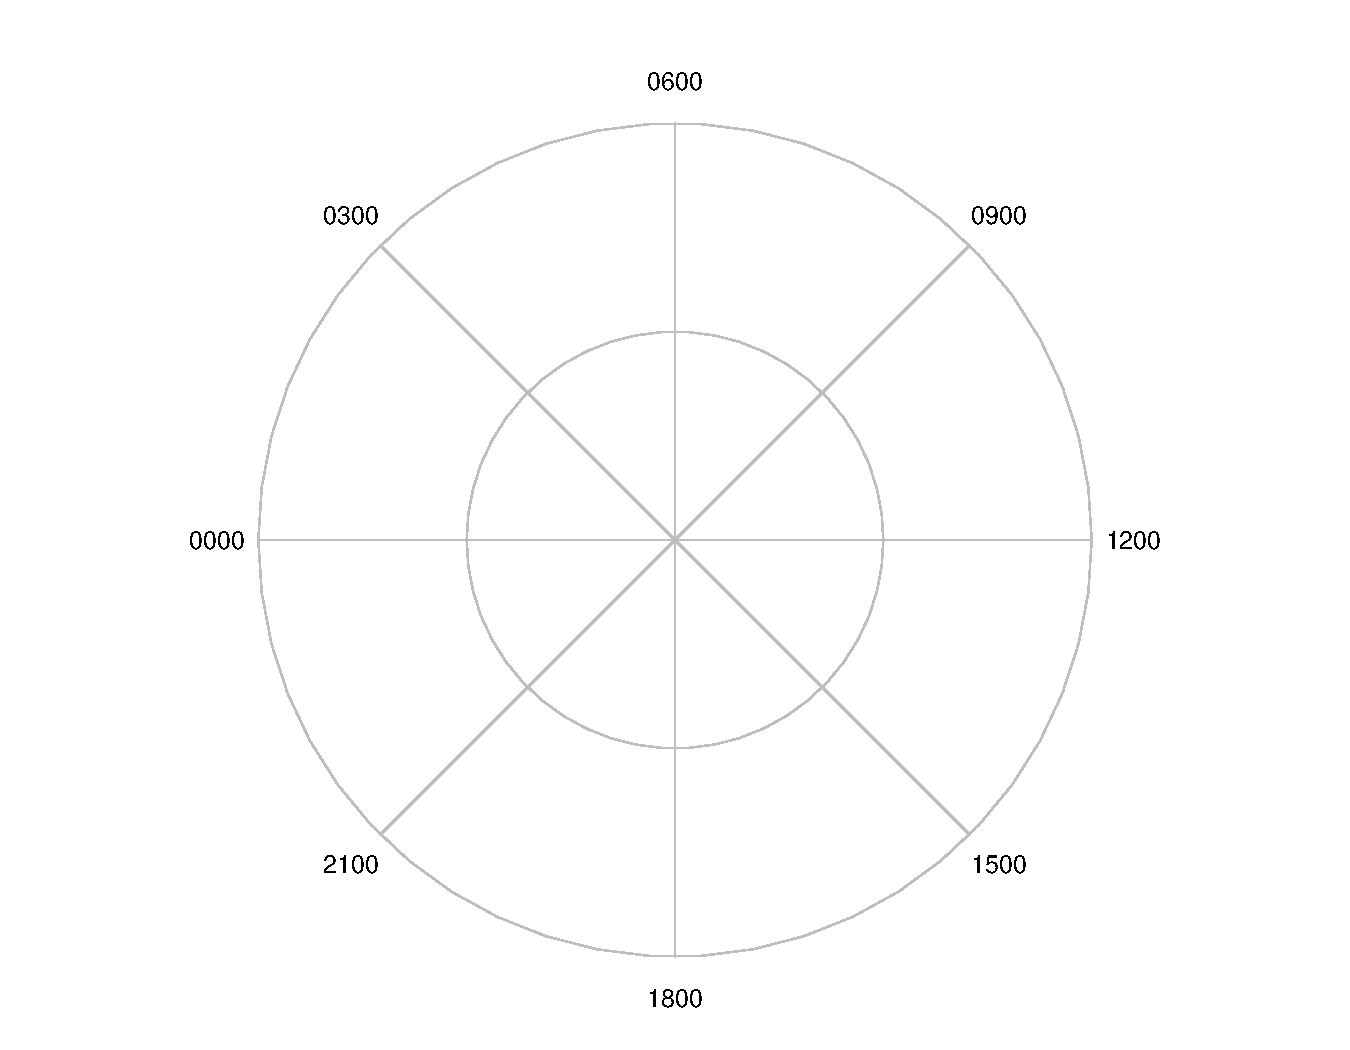
\includegraphics[width=0.9\linewidth]{_main_files/figure-latex/emptyDiel-1} 

}

\caption{An empty dielPlot().}\label{fig:emptyDiel}
\end{figure}

\hypertarget{emptyyearly}{%
\subsection{\texorpdfstring{\texttt{emptyYearly()}}{emptyYearly()}}\label{emptyyearly}}

The \texttt{emptyYearly()} function takes an option \texttt{year} parameter that automatically adjusts the grid positions for leap years, although the visual effect is marginal.

\begin{Shaded}
\begin{Highlighting}[]
\FunctionTok{emptyYearly}\NormalTok{(}\AttributeTok{year=}\DecValTok{2000}\NormalTok{)}
\end{Highlighting}
\end{Shaded}

\begin{figure}

{\centering 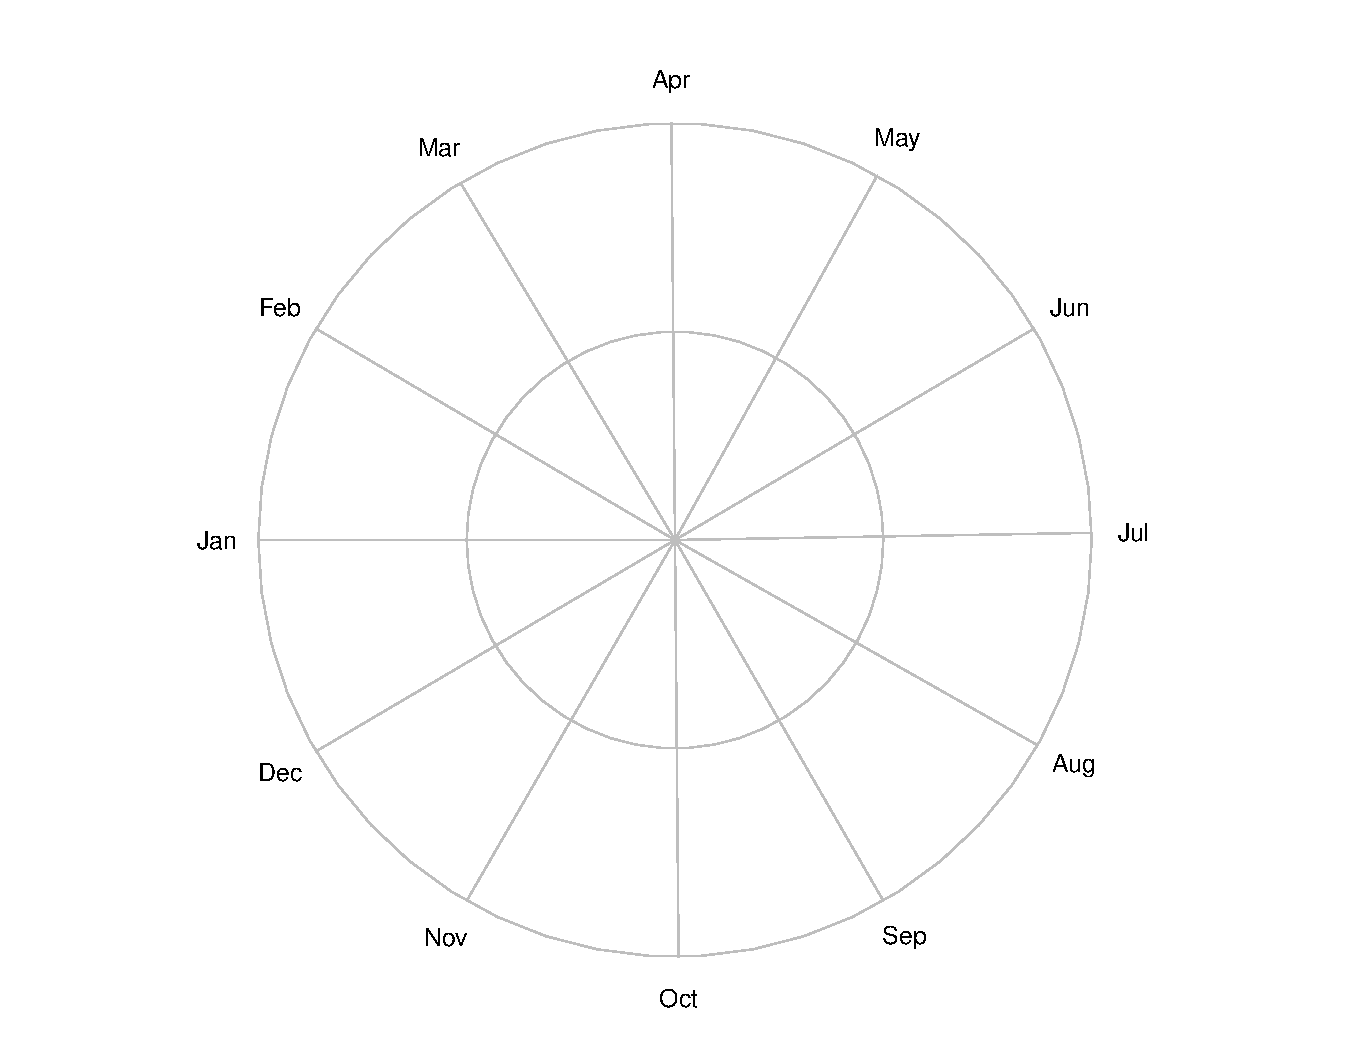
\includegraphics[width=0.9\linewidth]{_main_files/figure-latex/emptyYearly-1} 

}

\caption{An empty yearlyPlot().}\label{fig:emptyYearly}
\end{figure}

\hypertarget{adding-to-cyclical}{%
\section{Adding data to the visualisation}\label{adding-to-cyclical}}

\hypertarget{periodic-data-rings}{%
\subsection{Periodic data: rings}\label{periodic-data-rings}}

The ring functions (\texttt{dielRing()},\ldots) plot ring segments on top of a base cyclical plot. These rings are useful for showing typical periods of activity for a species, or events that happen continuously for a specified period of time.

By defaults the limits for the rings are \texttt{1,2} for use with a \emph{core} type plot, but this can be changed by specifying the \texttt{limits} parameter to the ring function. Similarly, the plot legend may be removed with the paramater \texttt{legend=FALSE}.

\hypertarget{dielrings}{%
\subsubsection{\texorpdfstring{\texttt{dielRings()}}{dielRings()}}\label{dielrings}}

\begin{Shaded}
\begin{Highlighting}[]
\NormalTok{names }\OtherTok{\textless{}{-}} \FunctionTok{c}\NormalTok{(}\StringTok{"activity 1"}\NormalTok{, }\StringTok{"activity 2"}\NormalTok{, }\StringTok{"activity 3"}\NormalTok{)}
\NormalTok{starts }\OtherTok{\textless{}{-}} \FunctionTok{c}\NormalTok{(}\StringTok{"0600"}\NormalTok{, }\StringTok{"0900"}\NormalTok{, }\StringTok{"1500"}\NormalTok{)}
\NormalTok{ends }\OtherTok{\textless{}{-}} \FunctionTok{c}\NormalTok{(}\StringTok{"1200"}\NormalTok{, }\StringTok{"1700"}\NormalTok{, }\StringTok{"1900"}\NormalTok{)}
\NormalTok{cols }\OtherTok{\textless{}{-}} \FunctionTok{c}\NormalTok{(}\StringTok{"red"}\NormalTok{, }\StringTok{"green"}\NormalTok{, }\StringTok{"blue"}\NormalTok{)}

\FunctionTok{dielPlot}\NormalTok{(}\StringTok{"2022{-}08{-}08"}\NormalTok{, }\AttributeTok{lat=}\DecValTok{53}\NormalTok{, }\AttributeTok{lon=}\FloatTok{0.1}\NormalTok{, }\AttributeTok{limits=}\FunctionTok{c}\NormalTok{(}\DecValTok{0}\NormalTok{,}\DecValTok{1}\NormalTok{))}
\FunctionTok{dielRings}\NormalTok{(names, starts, ends, }\AttributeTok{cols=}\NormalTok{cols)}
\end{Highlighting}
\end{Shaded}

\begin{figure}

{\centering 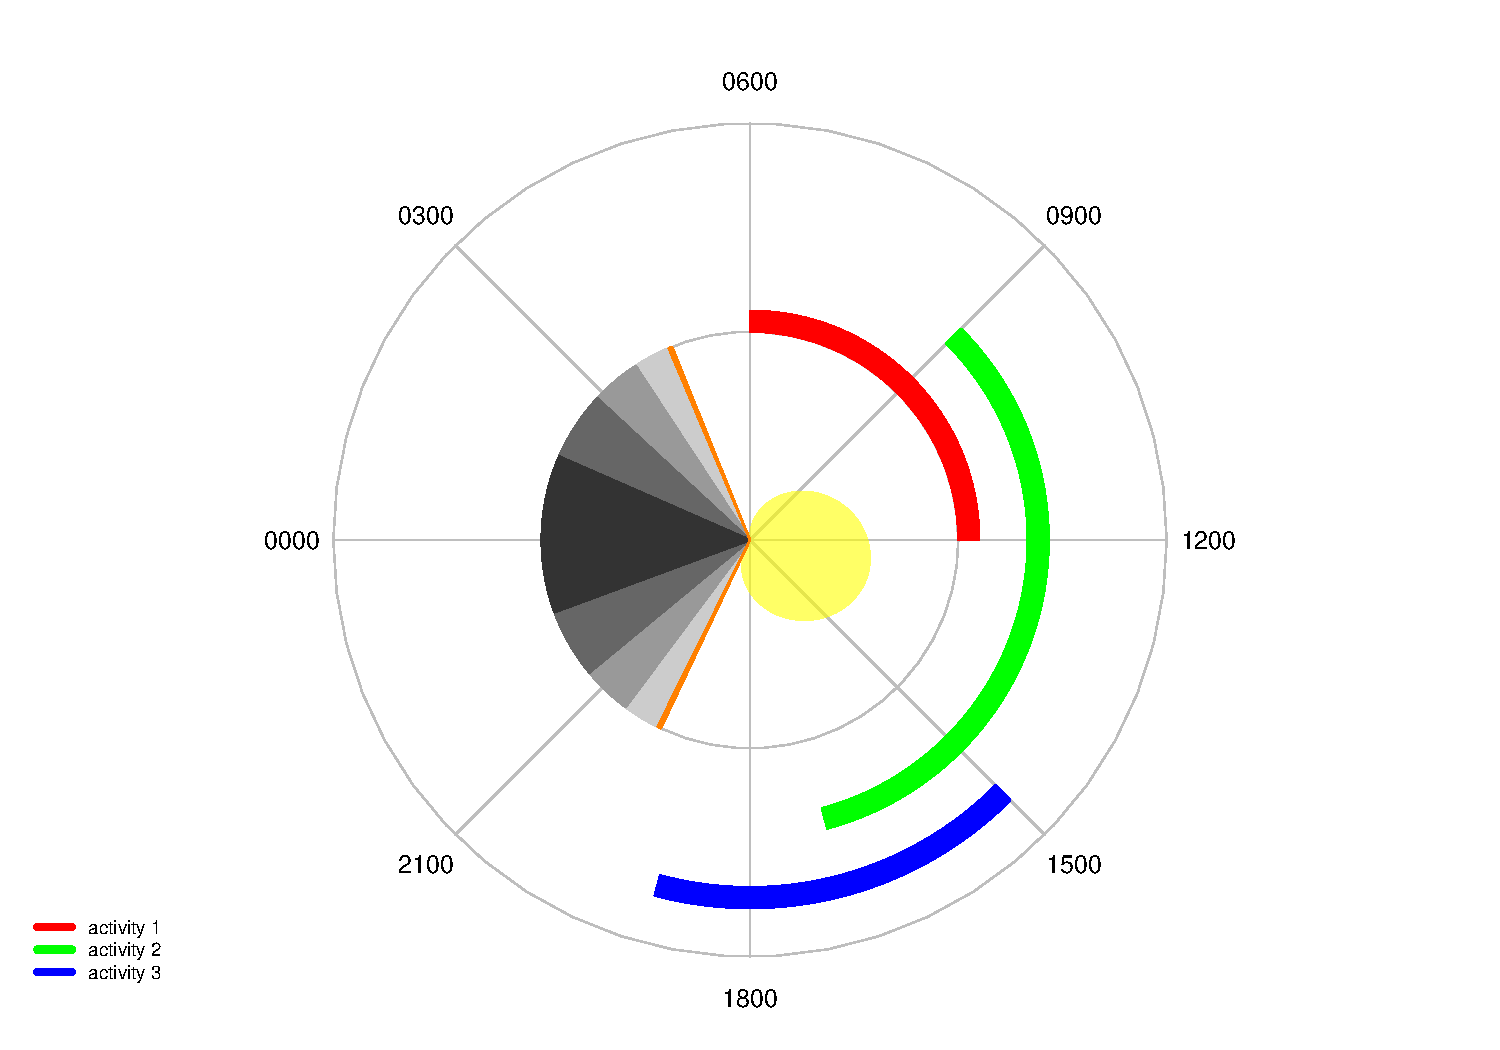
\includegraphics[width=0.9\linewidth]{_main_files/figure-latex/diel-plot-rings-1-1} 

}

\caption{A 'core' diel plot with diel rings.}\label{fig:diel-plot-rings-1}
\end{figure}

\begin{Shaded}
\begin{Highlighting}[]
\NormalTok{names }\OtherTok{\textless{}{-}} \FunctionTok{c}\NormalTok{(}\StringTok{"activity 1"}\NormalTok{, }\StringTok{"activity 2"}\NormalTok{, }\StringTok{"activity 3"}\NormalTok{)}
\NormalTok{starts }\OtherTok{\textless{}{-}} \FunctionTok{c}\NormalTok{(}\StringTok{"0600"}\NormalTok{, }\StringTok{"0900"}\NormalTok{, }\StringTok{"1500"}\NormalTok{)}
\NormalTok{ends }\OtherTok{\textless{}{-}} \FunctionTok{c}\NormalTok{(}\StringTok{"1200"}\NormalTok{, }\StringTok{"1700"}\NormalTok{, }\StringTok{"1900"}\NormalTok{)}
\NormalTok{cols }\OtherTok{\textless{}{-}} \FunctionTok{c}\NormalTok{(}\StringTok{"red"}\NormalTok{, }\StringTok{"green"}\NormalTok{, }\StringTok{"blue"}\NormalTok{)}

\FunctionTok{dielPlot}\NormalTok{(}\StringTok{"2022{-}08{-}08"}\NormalTok{, }\AttributeTok{lat=}\DecValTok{53}\NormalTok{, }\AttributeTok{lon=}\FloatTok{0.1}\NormalTok{, }\AttributeTok{limits=}\FunctionTok{c}\NormalTok{(}\DecValTok{1}\NormalTok{,}\DecValTok{2}\NormalTok{))}
\FunctionTok{dielRings}\NormalTok{(names, starts, ends, }\AttributeTok{cols=}\NormalTok{cols, }\AttributeTok{limits=}\FunctionTok{c}\NormalTok{(}\DecValTok{0}\NormalTok{,}\DecValTok{1}\NormalTok{))}
\end{Highlighting}
\end{Shaded}

\begin{figure}

{\centering 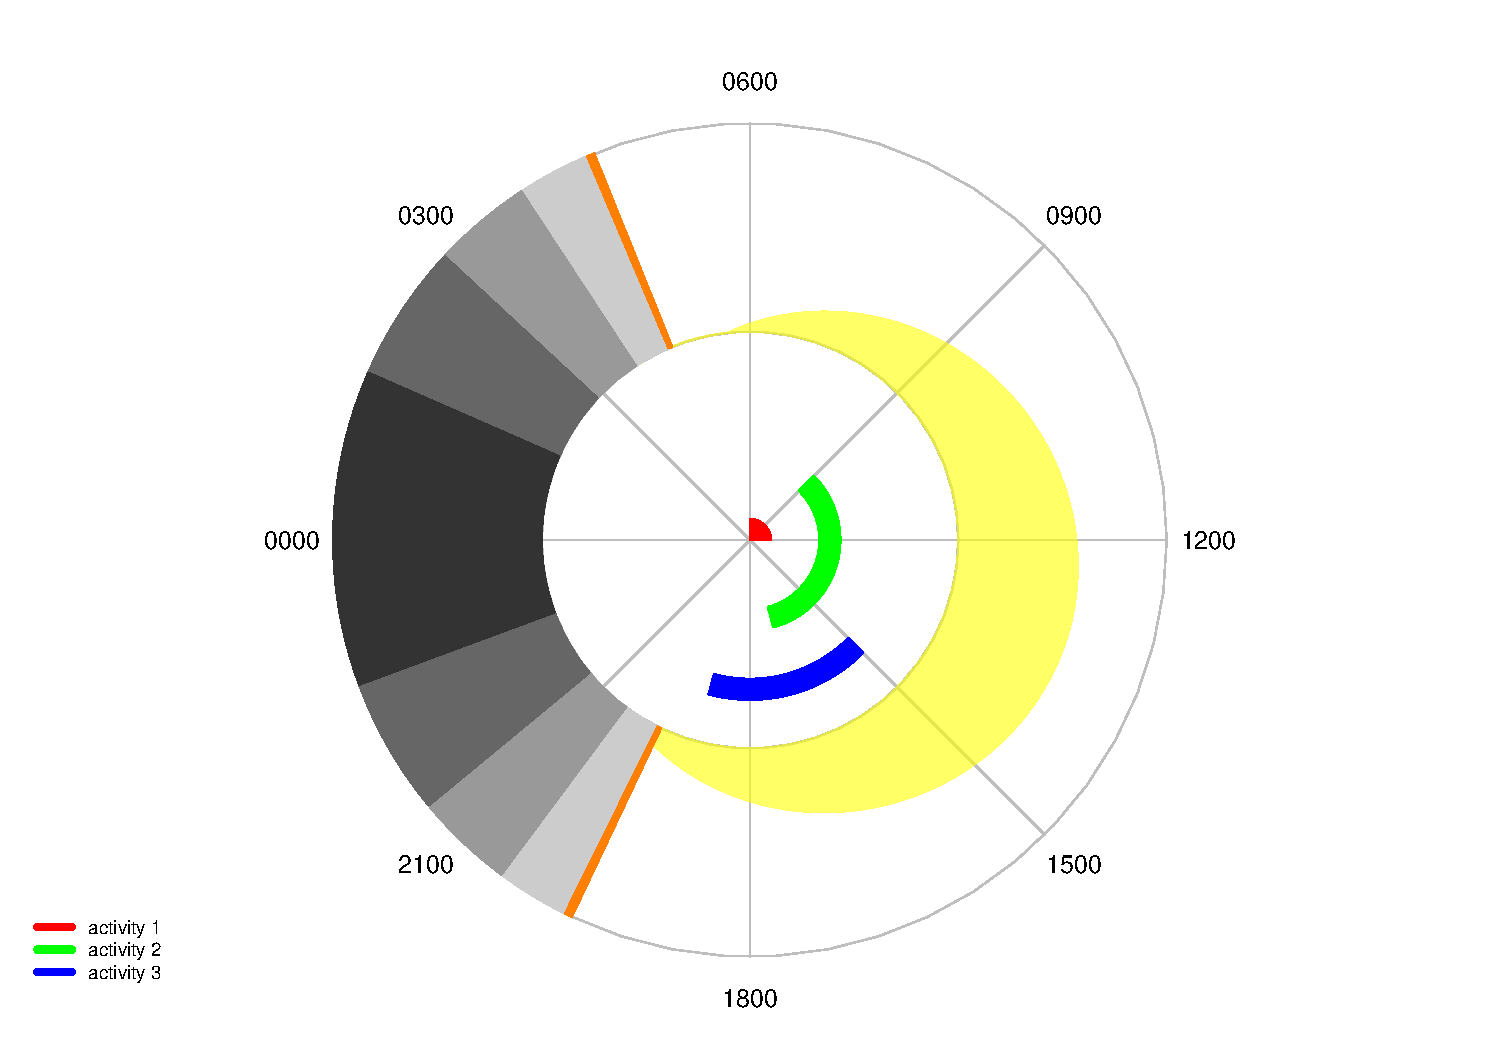
\includegraphics[width=0.9\linewidth]{_main_files/figure-latex/diel-plot-rings-2-1} 

}

\caption{A 'ring' diel plot with diel rings.}\label{fig:diel-plot-rings-2}
\end{figure}

\hypertarget{periodic-data-horizons}{%
\subsection{Periodic data: horizons}\label{periodic-data-horizons}}

In this example we will plot the average monthly minimum and maximum temperatures for Lyme Regis, UK onto a \texttt{yearlyPlot()}. This example introduces three small helper functions; \texttt{yearlyLabels()}, \texttt{yearlyPositions()} and \texttt{circularise()}.

\hypertarget{yearlylabels-and-yearlypositions}{%
\subsubsection{\texorpdfstring{\texttt{yearlyLabels()} and \texttt{yearlyPositions}}{yearlyLabels() and yearlyPositions}}\label{yearlylabels-and-yearlypositions}}

These two functions are closely related, and used internally by \texttt{SonicScrewdriveR} to label a yearly plot.

\begin{Shaded}
\begin{Highlighting}[]
\FunctionTok{yearlyLabels}\NormalTok{()}
\end{Highlighting}
\end{Shaded}

\begin{verbatim}
##  [1] "Jan" "Feb" "Mar" "Apr" "May" "Jun" "Jul" "Aug" "Sep" "Oct" "Nov" "Dec"
\end{verbatim}

The related \texttt{yearlyPositions()} gives angular positions for the data around the plot (in radians).

\begin{Shaded}
\begin{Highlighting}[]
\FunctionTok{yearlyPositions}\NormalTok{(}\AttributeTok{year=}\DecValTok{2022}\NormalTok{)}
\end{Highlighting}
\end{Shaded}

\begin{verbatim}
##  [1] 0.0000000 0.5336404 1.0156382 1.5492786 2.0657048 2.5993452 3.1157713
##  [8] 3.6494117 4.1830521 4.6994783 5.2331187 5.7495449
\end{verbatim}

The temperature data we have for Lyme Regis is monthly, however we would like to plot the values at the middle of the respective month. For this we add the parameter \texttt{format="mid-month"} to get the appropriate radial angles.

\begin{Shaded}
\begin{Highlighting}[]
\FunctionTok{yearlyPositions}\NormalTok{(}\AttributeTok{year=}\DecValTok{2022}\NormalTok{, }\AttributeTok{format=}\StringTok{"mid{-}months"}\NormalTok{)}
\end{Highlighting}
\end{Shaded}

\begin{verbatim}
##  [1] 0.2668202 0.7746393 1.2824584 1.8074917 2.3325250 2.8575582 3.3825915
##  [8] 3.9162319 4.4412652 4.9662985 5.4913318 5.9733296
\end{verbatim}

If we now plot this data we see that the output is not quite a complete ring or horizon data as we might have expected.

\begin{Shaded}
\begin{Highlighting}[]
\CommentTok{\# Temperature data for Lyme Regis}
\NormalTok{t\_min }\OtherTok{\textless{}{-}} \FunctionTok{c}\NormalTok{(}\DecValTok{3}\NormalTok{, }\FloatTok{2.7}\NormalTok{, }\FloatTok{3.4}\NormalTok{, }\FloatTok{5.2}\NormalTok{, }\FloatTok{8.2}\NormalTok{, }\FloatTok{11.2}\NormalTok{, }\FloatTok{13.1}\NormalTok{, }\DecValTok{13}\NormalTok{, }\FloatTok{14.4}\NormalTok{, }\FloatTok{9.2}\NormalTok{, }\FloatTok{5.8}\NormalTok{, }\FloatTok{3.8}\NormalTok{)}
\NormalTok{t\_max }\OtherTok{\textless{}{-}} \FunctionTok{c}\NormalTok{(}\FloatTok{7.9}\NormalTok{,}\DecValTok{8}\NormalTok{, }\FloatTok{9.8}\NormalTok{, }\FloatTok{12.4}\NormalTok{, }\FloatTok{15.4}\NormalTok{, }\FloatTok{18.2}\NormalTok{, }\FloatTok{20.1}\NormalTok{, }\FloatTok{19.5}\NormalTok{, }\FloatTok{17.8}\NormalTok{, }\FloatTok{14.4}\NormalTok{, }\FloatTok{10.6}\NormalTok{, }\FloatTok{8.4}\NormalTok{)}

\CommentTok{\# Scale the data}
\NormalTok{sf }\OtherTok{\textless{}{-}} \FunctionTok{max}\NormalTok{(t\_max)}
\NormalTok{t\_min }\OtherTok{\textless{}{-}}\NormalTok{ t\_min}\SpecialCharTok{/}\NormalTok{sf}
\NormalTok{t\_max }\OtherTok{\textless{}{-}}\NormalTok{ t\_max}\SpecialCharTok{/}\NormalTok{sf}

\NormalTok{angles }\OtherTok{\textless{}{-}} \FunctionTok{yearlyPositions}\NormalTok{(}\AttributeTok{format=}\StringTok{"mid{-}months"}\NormalTok{)}

\FunctionTok{yearlyPlot}\NormalTok{(}\AttributeTok{lat=}\FloatTok{50.7}\NormalTok{, }\AttributeTok{lon=}\SpecialCharTok{{-}}\FloatTok{2.9}\NormalTok{)}
\FunctionTok{radialPolygon}\NormalTok{(angles, angles, t\_min, t\_max, }\AttributeTok{col=}\StringTok{"orange"}\NormalTok{)}
\end{Highlighting}
\end{Shaded}

\begin{figure}

{\centering 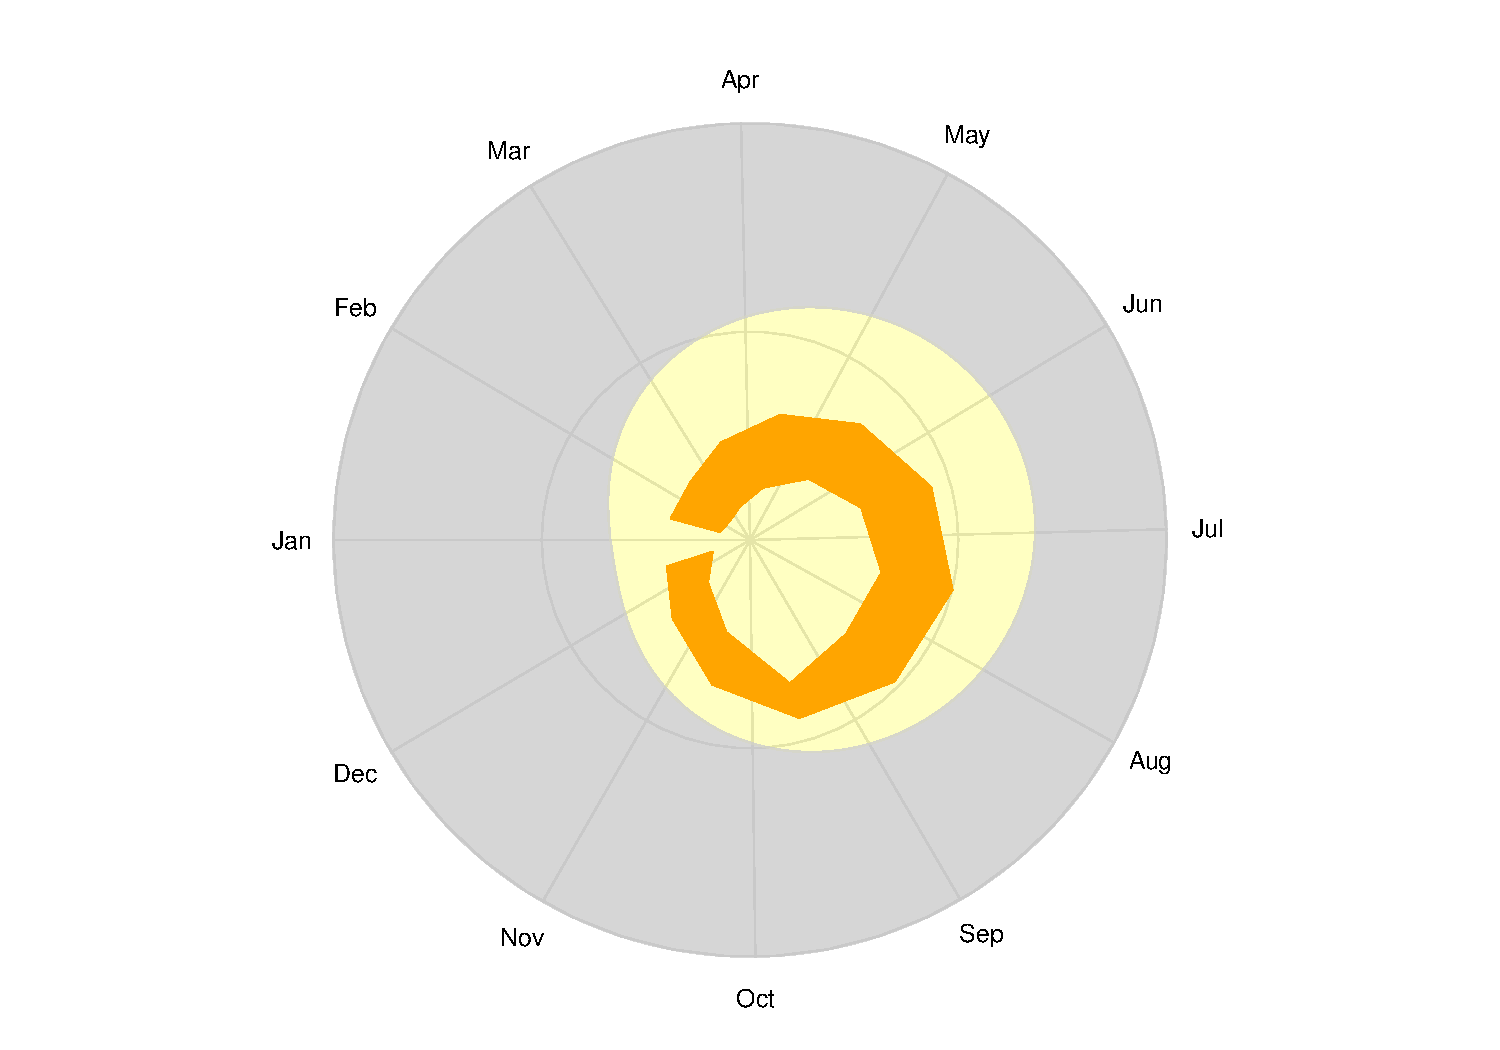
\includegraphics[width=0.9\linewidth]{_main_files/figure-latex/lyme-temp-1-1} 

}

\caption{Horizon data plot without circularise().}\label{fig:lyme-temp-1}
\end{figure}

\hypertarget{circularise}{%
\subsubsection{\texorpdfstring{\texttt{circularise()}}{circularise()}}\label{circularise}}

In order to join the horizons into a complete ring we can use the \texttt{circularise()} function on the angle and temperature vectors.

\begin{Shaded}
\begin{Highlighting}[]
\CommentTok{\# Temperature data for Lyme Regis}
\NormalTok{t\_min }\OtherTok{\textless{}{-}} \FunctionTok{c}\NormalTok{(}\DecValTok{3}\NormalTok{, }\FloatTok{2.7}\NormalTok{, }\FloatTok{3.4}\NormalTok{, }\FloatTok{5.2}\NormalTok{, }\FloatTok{8.2}\NormalTok{, }\FloatTok{11.2}\NormalTok{, }\FloatTok{13.1}\NormalTok{, }\DecValTok{13}\NormalTok{, }\FloatTok{14.4}\NormalTok{, }\FloatTok{9.2}\NormalTok{, }\FloatTok{5.8}\NormalTok{, }\FloatTok{3.8}\NormalTok{)}
\NormalTok{t\_max }\OtherTok{\textless{}{-}} \FunctionTok{c}\NormalTok{(}\FloatTok{7.9}\NormalTok{,}\DecValTok{8}\NormalTok{, }\FloatTok{9.8}\NormalTok{, }\FloatTok{12.4}\NormalTok{, }\FloatTok{15.4}\NormalTok{, }\FloatTok{18.2}\NormalTok{, }\FloatTok{20.1}\NormalTok{, }\FloatTok{19.5}\NormalTok{, }\FloatTok{17.8}\NormalTok{, }\FloatTok{14.4}\NormalTok{, }\FloatTok{10.6}\NormalTok{, }\FloatTok{8.4}\NormalTok{)}

\CommentTok{\# Scale the data}
\NormalTok{sf }\OtherTok{\textless{}{-}} \FunctionTok{max}\NormalTok{(t\_max)}
\NormalTok{t\_min }\OtherTok{\textless{}{-}}\NormalTok{ t\_min}\SpecialCharTok{/}\NormalTok{sf}
\NormalTok{t\_max }\OtherTok{\textless{}{-}}\NormalTok{ t\_max}\SpecialCharTok{/}\NormalTok{sf}

\NormalTok{angles }\OtherTok{\textless{}{-}} \FunctionTok{yearlyPositions}\NormalTok{(}\AttributeTok{format=}\StringTok{"mid{-}months"}\NormalTok{)}

\CommentTok{\# Circularise}
\NormalTok{t\_min }\OtherTok{\textless{}{-}} \FunctionTok{circularise}\NormalTok{(t\_min)}
\NormalTok{t\_max }\OtherTok{\textless{}{-}} \FunctionTok{circularise}\NormalTok{(t\_max)}
\NormalTok{angles }\OtherTok{\textless{}{-}} \FunctionTok{circularise}\NormalTok{(angles)}

\FunctionTok{yearlyPlot}\NormalTok{(}\AttributeTok{lat=}\FloatTok{50.7}\NormalTok{, }\AttributeTok{lon=}\SpecialCharTok{{-}}\FloatTok{2.9}\NormalTok{)}
\FunctionTok{radialPolygon}\NormalTok{(angles, angles, t\_min, t\_max, }\AttributeTok{col=}\StringTok{"orange"}\NormalTok{)}
\end{Highlighting}
\end{Shaded}

\begin{figure}

{\centering 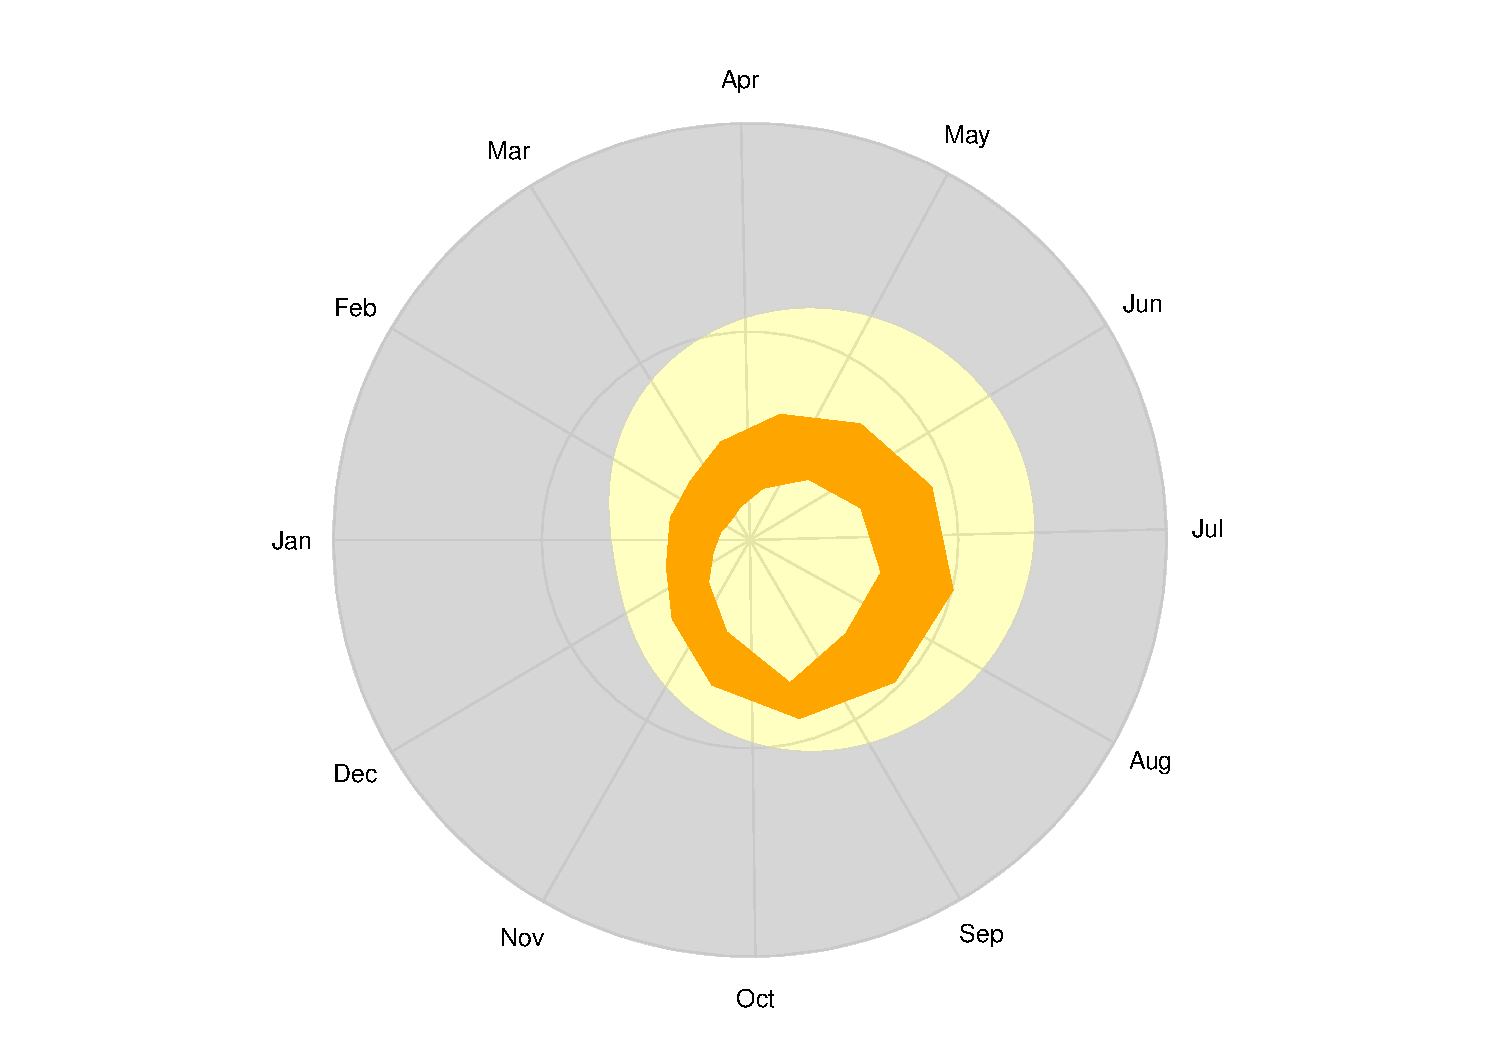
\includegraphics[width=0.9\linewidth]{_main_files/figure-latex/lyme-temp-2-1} 

}

\caption{Horizon data plot with circularise().}\label{fig:lyme-temp-2}
\end{figure}

\hypertarget{helper-functions}{%
\subsection{Helper functions}\label{helper-functions}}

\hypertarget{dielfraction}{%
\subsubsection{\texorpdfstring{\texttt{dielFraction()}}{dielFraction()}}\label{dielfraction}}

The \texttt{dielFraction()} function is used to convert a POSIX time, or a time in \texttt{HHMM} string format, into a radial fraction. This function is called by \texttt{dielPlot()} and \texttt{dielRings()}. By default the output is multiplied by 2π to output a position round a circle.

\begin{Shaded}
\begin{Highlighting}[]
\NormalTok{time }\OtherTok{\textless{}{-}} \FunctionTok{Sys.time}\NormalTok{()}
\FunctionTok{print}\NormalTok{(time)}
\end{Highlighting}
\end{Shaded}

\begin{verbatim}
## [1] "2022-10-29 10:10:33 BST"
\end{verbatim}

\begin{Shaded}
\begin{Highlighting}[]
\NormalTok{frac }\OtherTok{\textless{}{-}} \FunctionTok{dielFraction}\NormalTok{(time)}
\FunctionTok{print}\NormalTok{(frac)}
\end{Highlighting}
\end{Shaded}

\begin{verbatim}
## [1] 2.664088
\end{verbatim}

The raw fraction can be specified using the parameter \texttt{unit="fraction"}.

\begin{Shaded}
\begin{Highlighting}[]
\NormalTok{time }\OtherTok{\textless{}{-}} \FunctionTok{Sys.time}\NormalTok{()}
\FunctionTok{print}\NormalTok{(time)}
\end{Highlighting}
\end{Shaded}

\begin{verbatim}
## [1] "2022-10-29 10:10:33 BST"
\end{verbatim}

\begin{Shaded}
\begin{Highlighting}[]
\NormalTok{frac }\OtherTok{\textless{}{-}} \FunctionTok{dielFraction}\NormalTok{(time, }\AttributeTok{unit=}\StringTok{"fraction"}\NormalTok{)}
\FunctionTok{print}\NormalTok{(frac)}
\end{Highlighting}
\end{Shaded}

\begin{verbatim}
## [1] 0.4240029
\end{verbatim}

\hypertarget{yearlyfraction}{%
\subsubsection{\texorpdfstring{\texttt{yearlyFraction()}}{yearlyFraction()}}\label{yearlyfraction}}

Similarly to \texttt{dielFraction()}, \texttt{yearlyFraction()} by default returns a fraction of a cycle. It can take either a number representing a day of the year, or an object that can be coerced into \texttt{POSIXlt} format.

\begin{Shaded}
\begin{Highlighting}[]
\NormalTok{frac }\OtherTok{\textless{}{-}} \FunctionTok{yearlyFraction}\NormalTok{(}\DecValTok{31}\NormalTok{, }\AttributeTok{input=}\StringTok{"day"}\NormalTok{)}
\FunctionTok{print}\NormalTok{(frac)}
\end{Highlighting}
\end{Shaded}

\begin{verbatim}
## [1] 0.5336404
\end{verbatim}

\begin{Shaded}
\begin{Highlighting}[]
\NormalTok{date }\OtherTok{\textless{}{-}} \FunctionTok{Sys.Date}\NormalTok{()}
\FunctionTok{print}\NormalTok{(date)}
\end{Highlighting}
\end{Shaded}

\begin{verbatim}
## [1] "2022-10-29"
\end{verbatim}

\begin{Shaded}
\begin{Highlighting}[]
\NormalTok{frac }\OtherTok{\textless{}{-}} \FunctionTok{yearlyFraction}\NormalTok{(date, }\AttributeTok{input=}\StringTok{"POSIXlt"}\NormalTok{)}
\FunctionTok{print}\NormalTok{(frac)}
\end{Highlighting}
\end{Shaded}

\begin{verbatim}
## [1] 5.181476
\end{verbatim}

\hypertarget{interactive-plots}{%
\section{Interactive Plots}\label{interactive-plots}}

These plots can be used to create Shiny apps

\begin{itemize}
\tightlist
\item
  \href{https://shiny.ebaker.me.uk/shiny-diel/}{shiny-diel} is an example that shows diel plots for a number of locations, and can be animated using the play button under the date slider.
\end{itemize}

\hypertarget{displaying-annotations}{%
\chapter{Displaying annotations}\label{displaying-annotations}}

\hypertarget{shiny-interactive-web-apps}{%
\chapter{Shiny: Interactive Web Apps}\label{shiny-interactive-web-apps}}

\hypertarget{the-future}{%
\chapter{The Future}\label{the-future}}

\hypertarget{acknowledgements}{%
\chapter{Acknowledgements}\label{acknowledgements}}

For discussions around visualisation as part of the Urban Nature Project: Chris Raper, John Tweddle.

Bruce Miller provided valuable feedback during the development of the zcjs visualisation tools for zero-crossing files.

The \texttt{SonicScrewdriveR} package was initially developed as part of the Leverhulme Trust funded Automated Acoustic Observatories project at the University of York, and development has continued as part of the Urban Nature Project at the Natural History Museum.

  \bibliography{book.bib,packages.bib}

\end{document}
